\def\secforfig{appendices/jet-level-trigger-sf}
\def\figsversion{V1}

%\begin{figure}[ht]
%    \centering
%    \subfloat[1st jet at L1]{\label{fig:trigSF16-1b0j-L1-1st}%
%            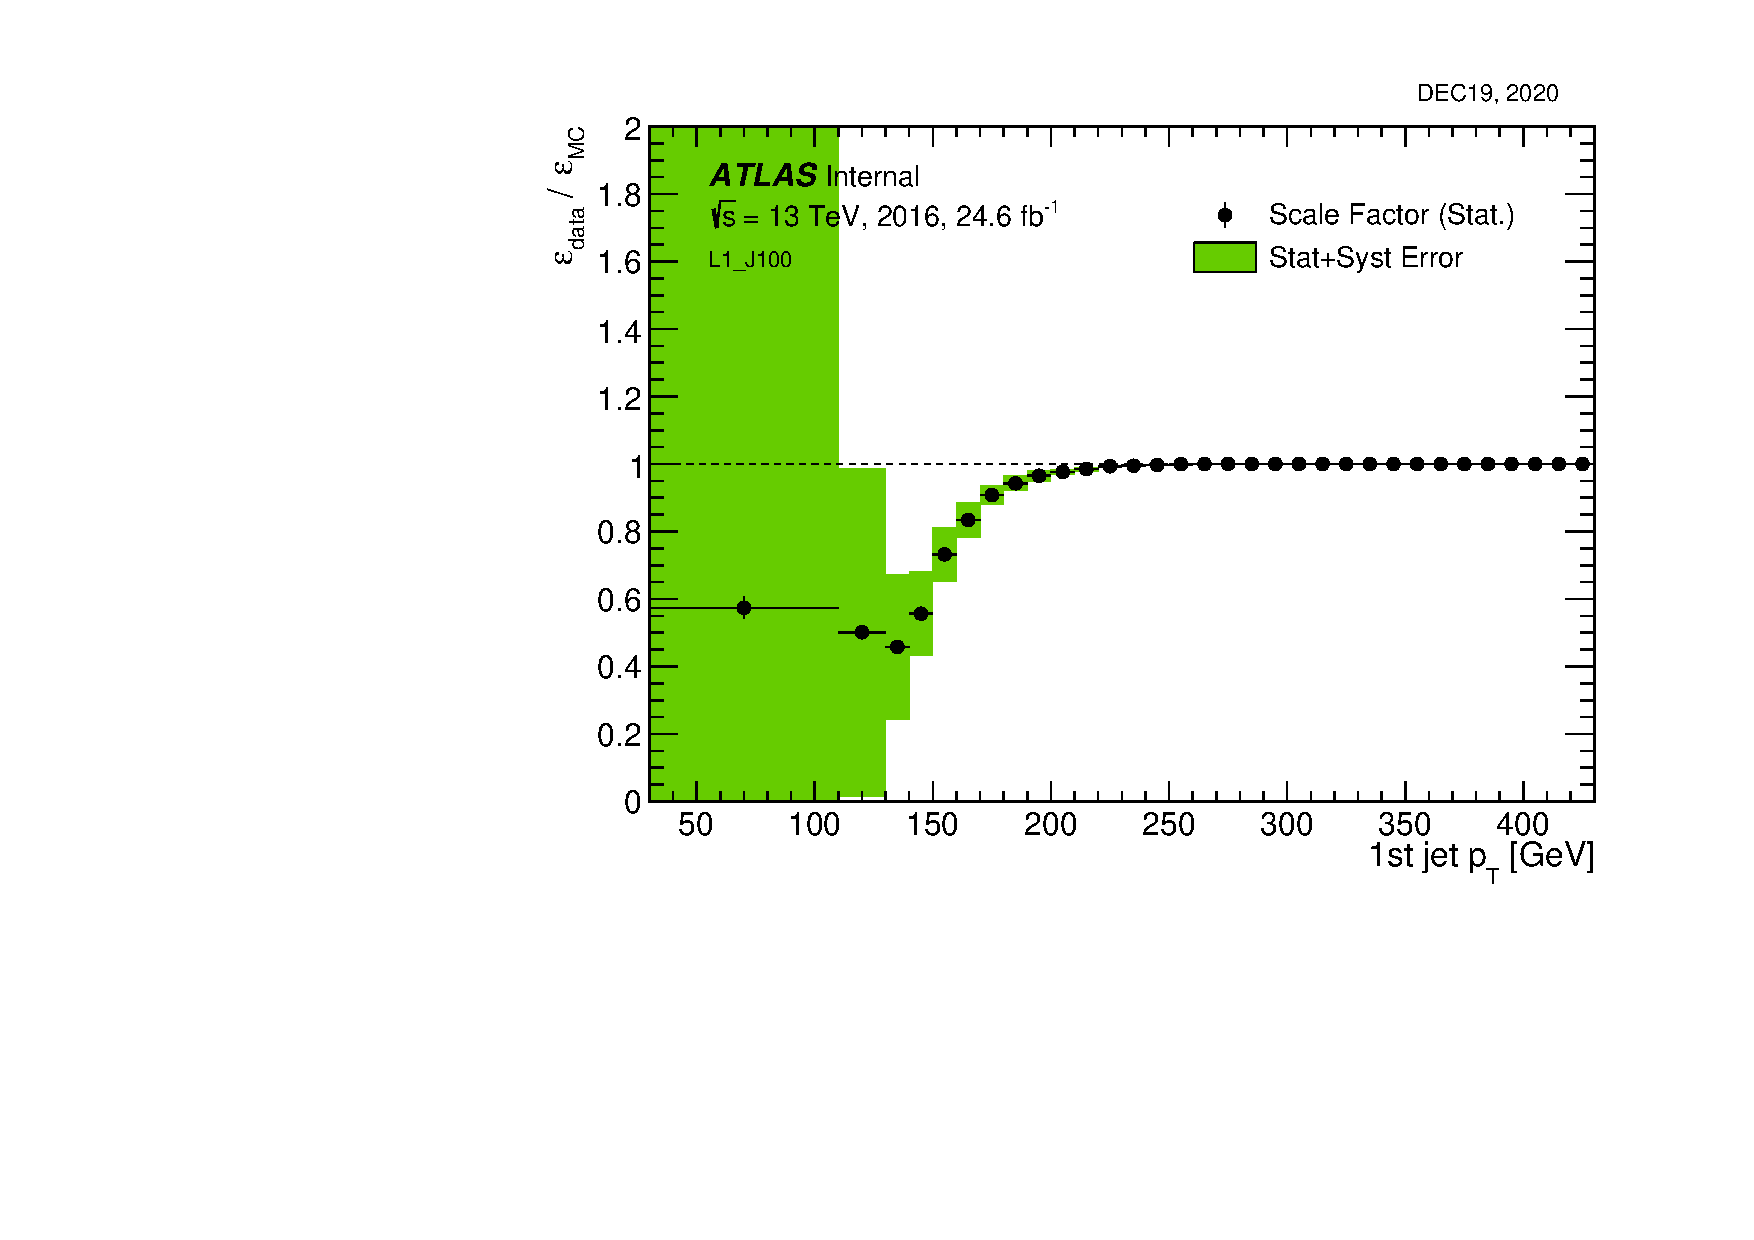
\includegraphics[width=0.25\textwidth]{\figpath{L1SF/2016/trigSF16-1b0j-L1-1st.pdf}}
%    }
%
%    \subfloat[1st jet at HLT]{\label{fig:trigSF16-1b0j-HLT-1st}%
%            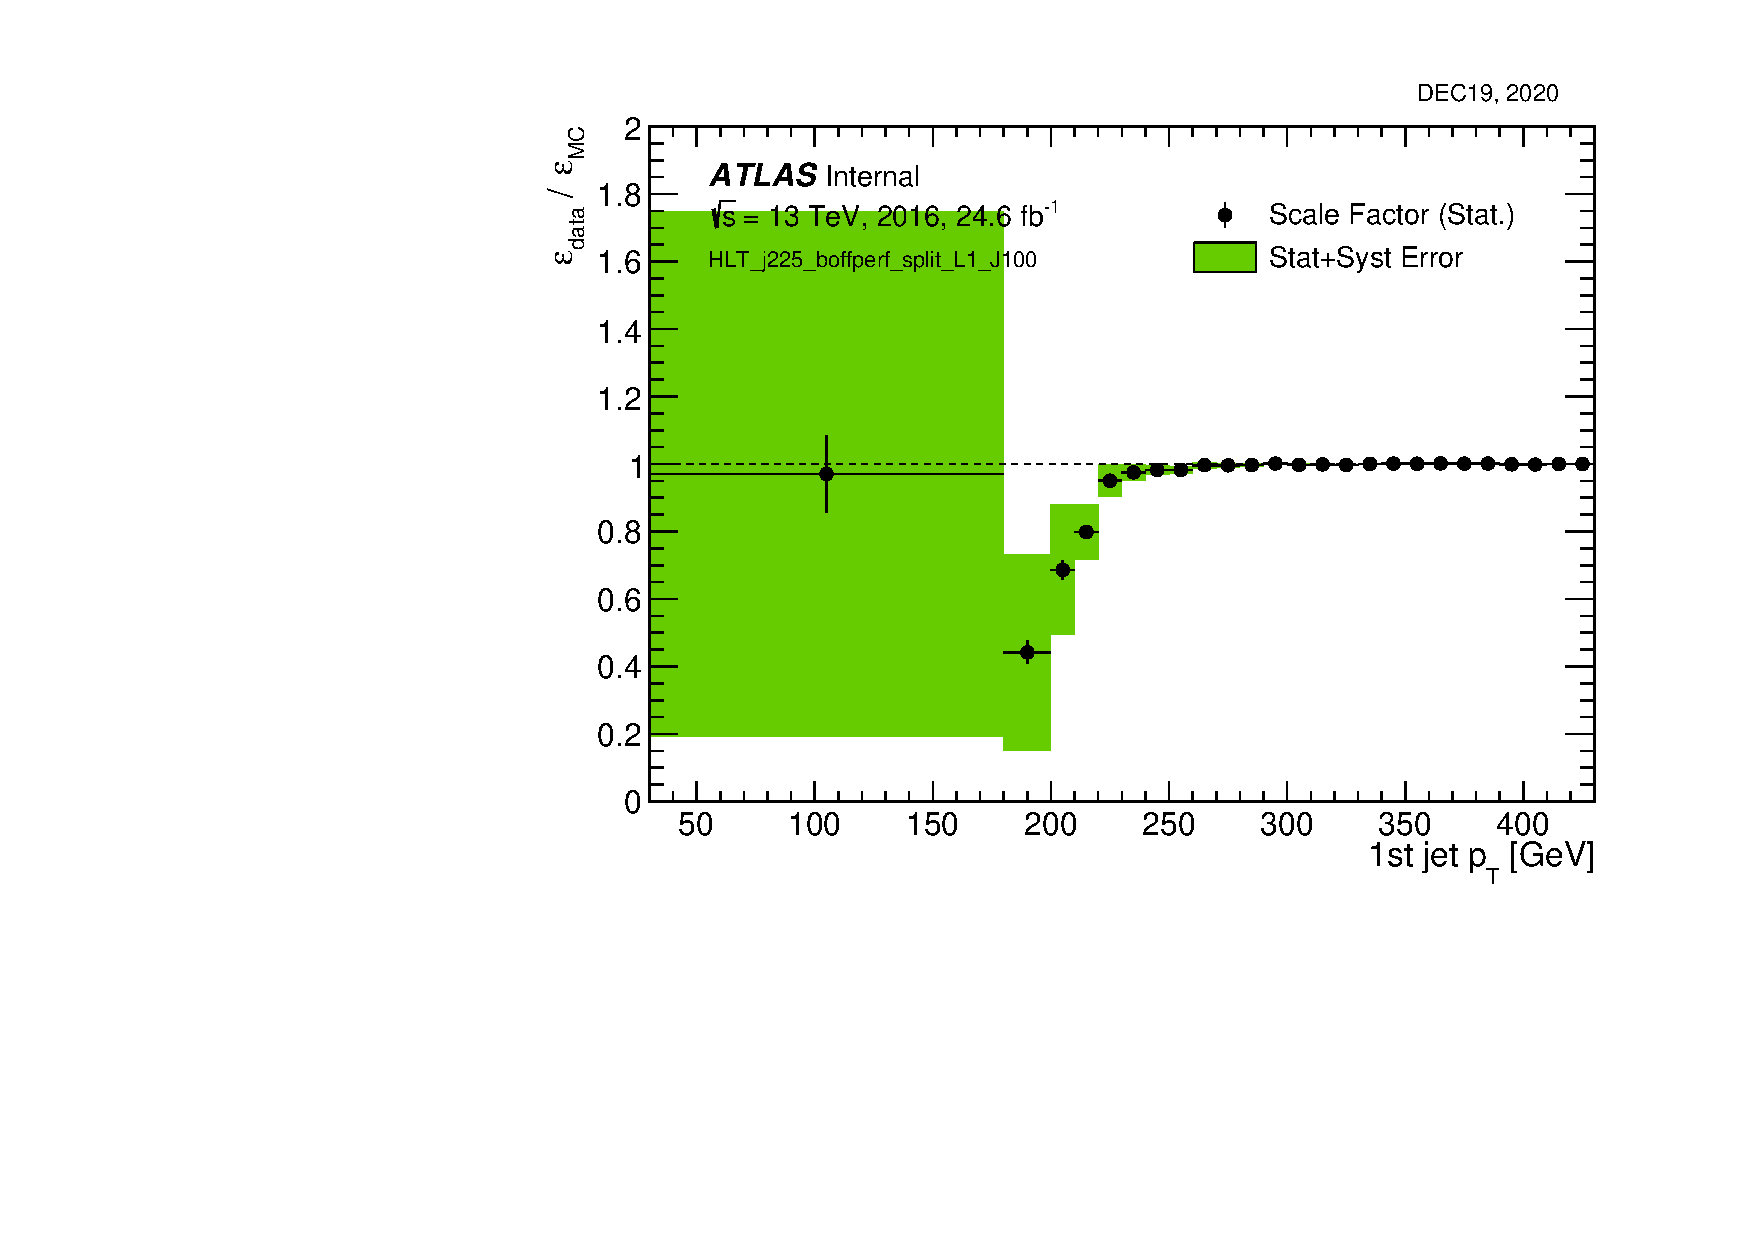
\includegraphics[width=0.25\textwidth]{\figpath{HLTSF/2016/trigSF16-1b0j-HLT-1st.pdf}}
%    }   
%    \caption{Jet-level scale factors of 2016 1b trigger as a function of offline jet \pt.
%             The Nth jet is ordered by online \et. }
%    \label{fig:trigSF16-1b0j}
%\end{figure}

\begin{figure}[ht]
    \centering
    \subfloat[1st jet at L1]{\label{fig:trigSF16-2b1j-L1-1st}%
            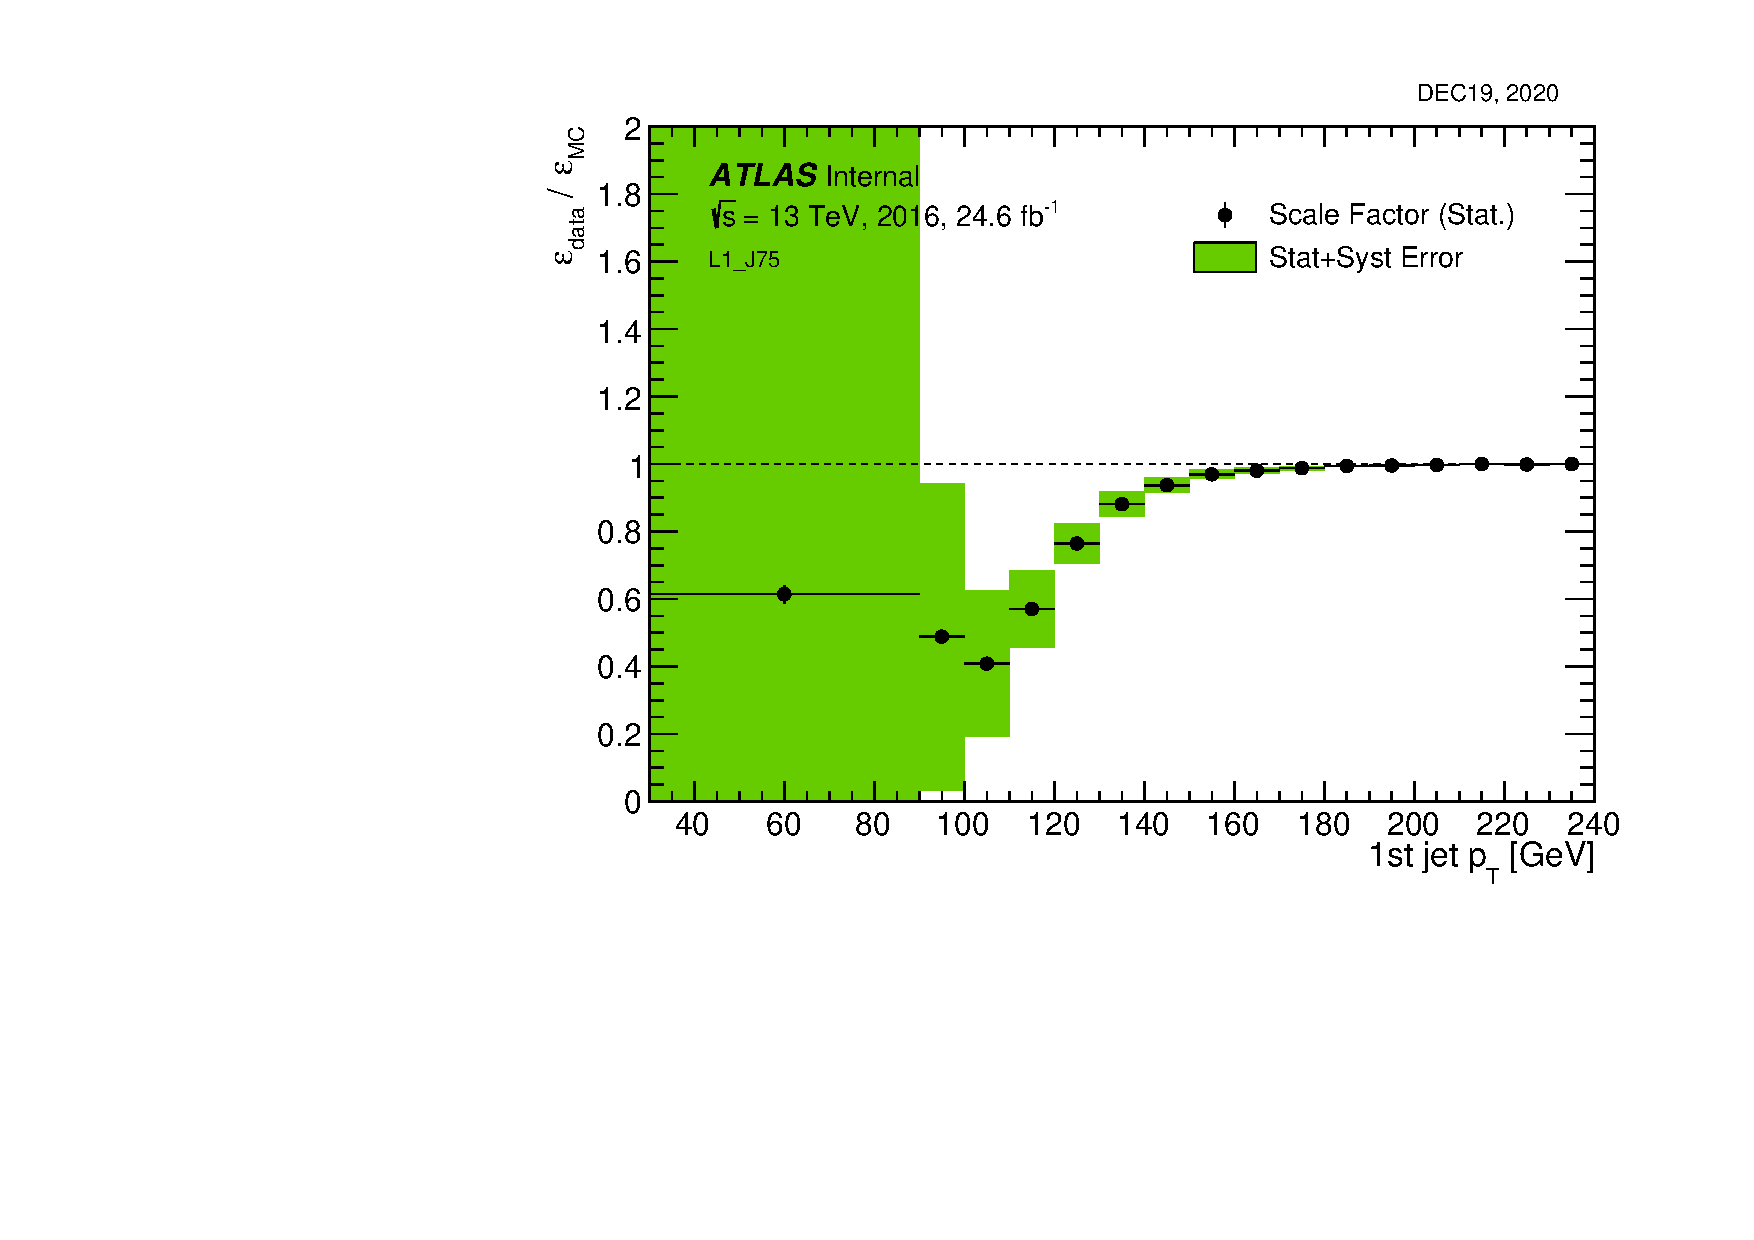
\includegraphics[width=0.25\textwidth]{\figpath{L1SF/2016/trigSF16-2b1j-L1-1st.pdf}}
    }   
    \subfloat[2nd jet at L1]{\label{fig:trigSF16-2b1j-L1-2nd}%
            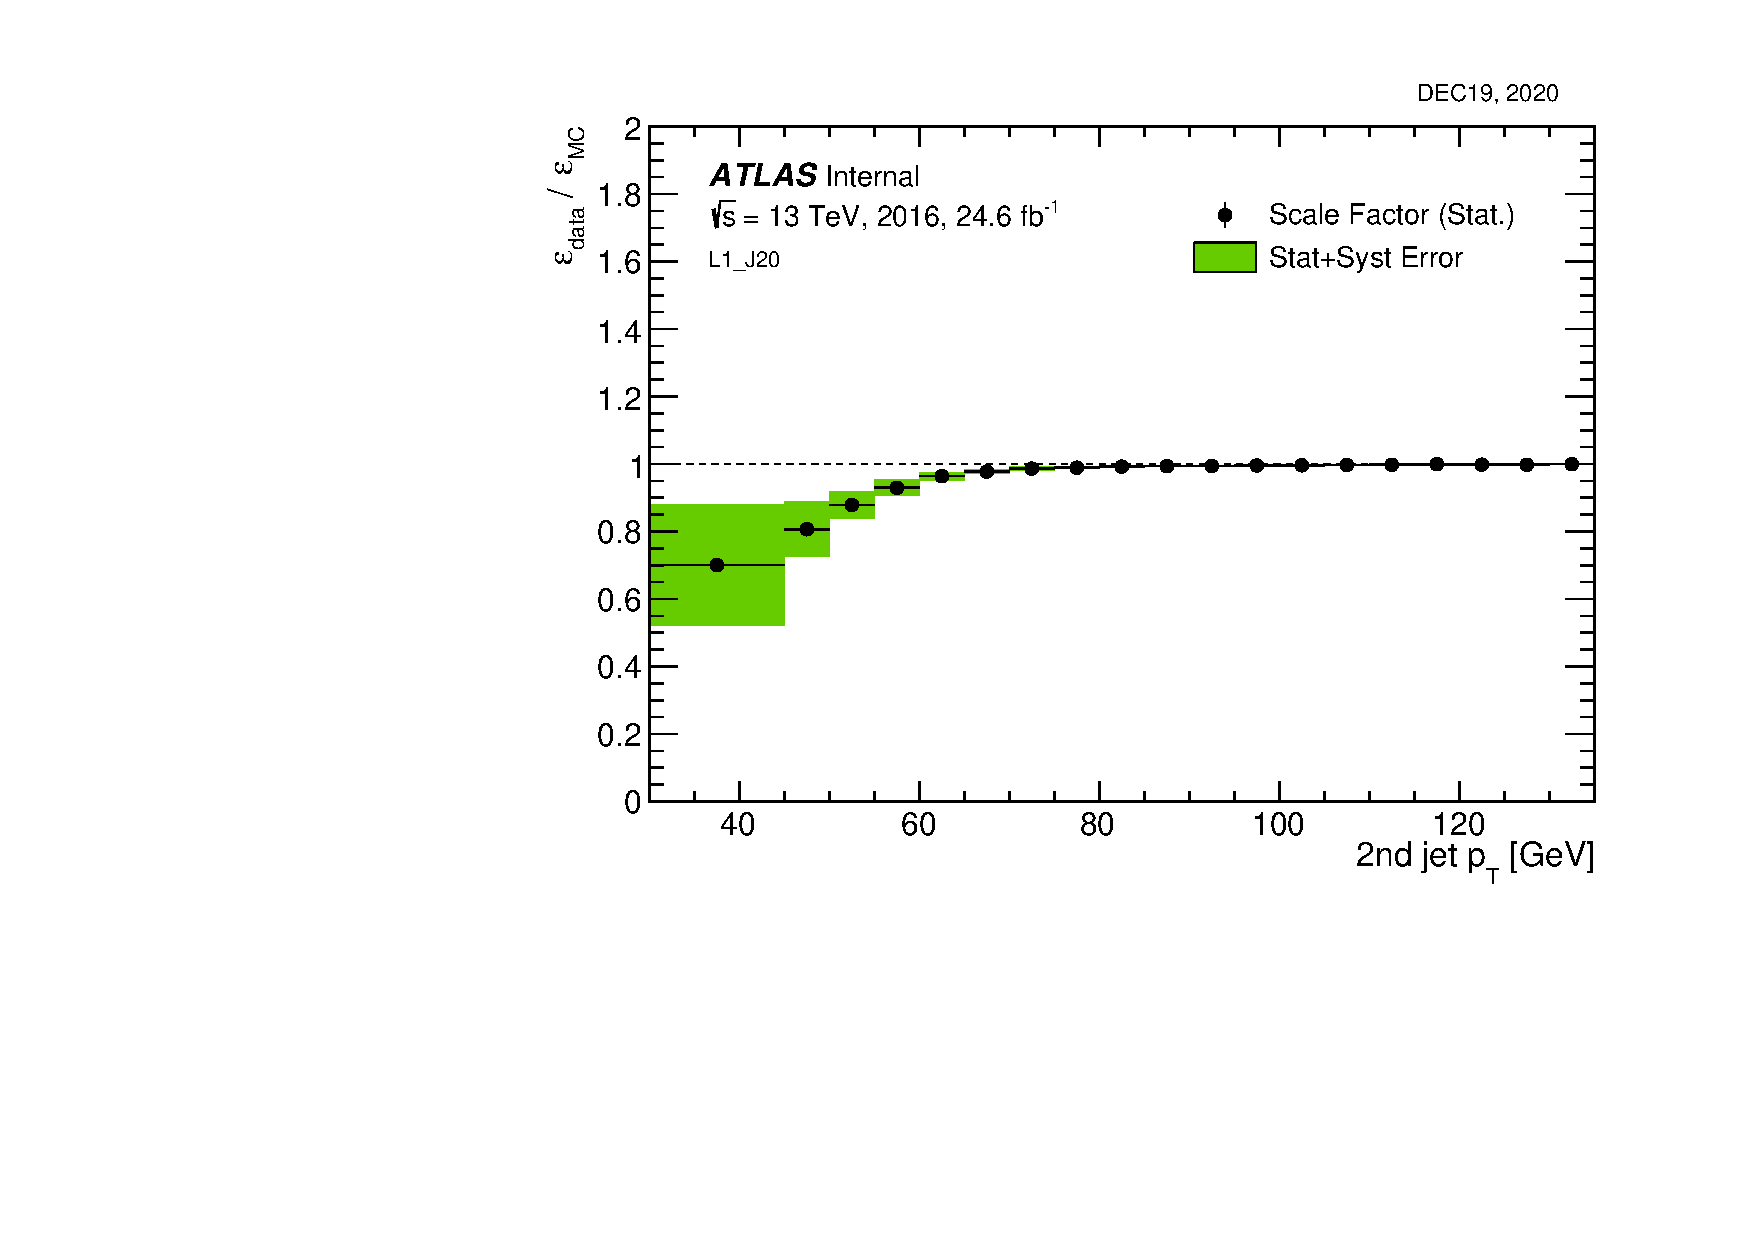
\includegraphics[width=0.25\textwidth]{\figpath{L1SF/2016/trigSF16-2b1j-L1-2nd.pdf}}
    }   
    \subfloat[3rd jet at L1]{\label{fig:trigSF16-2b1j-L1-3rd}%
            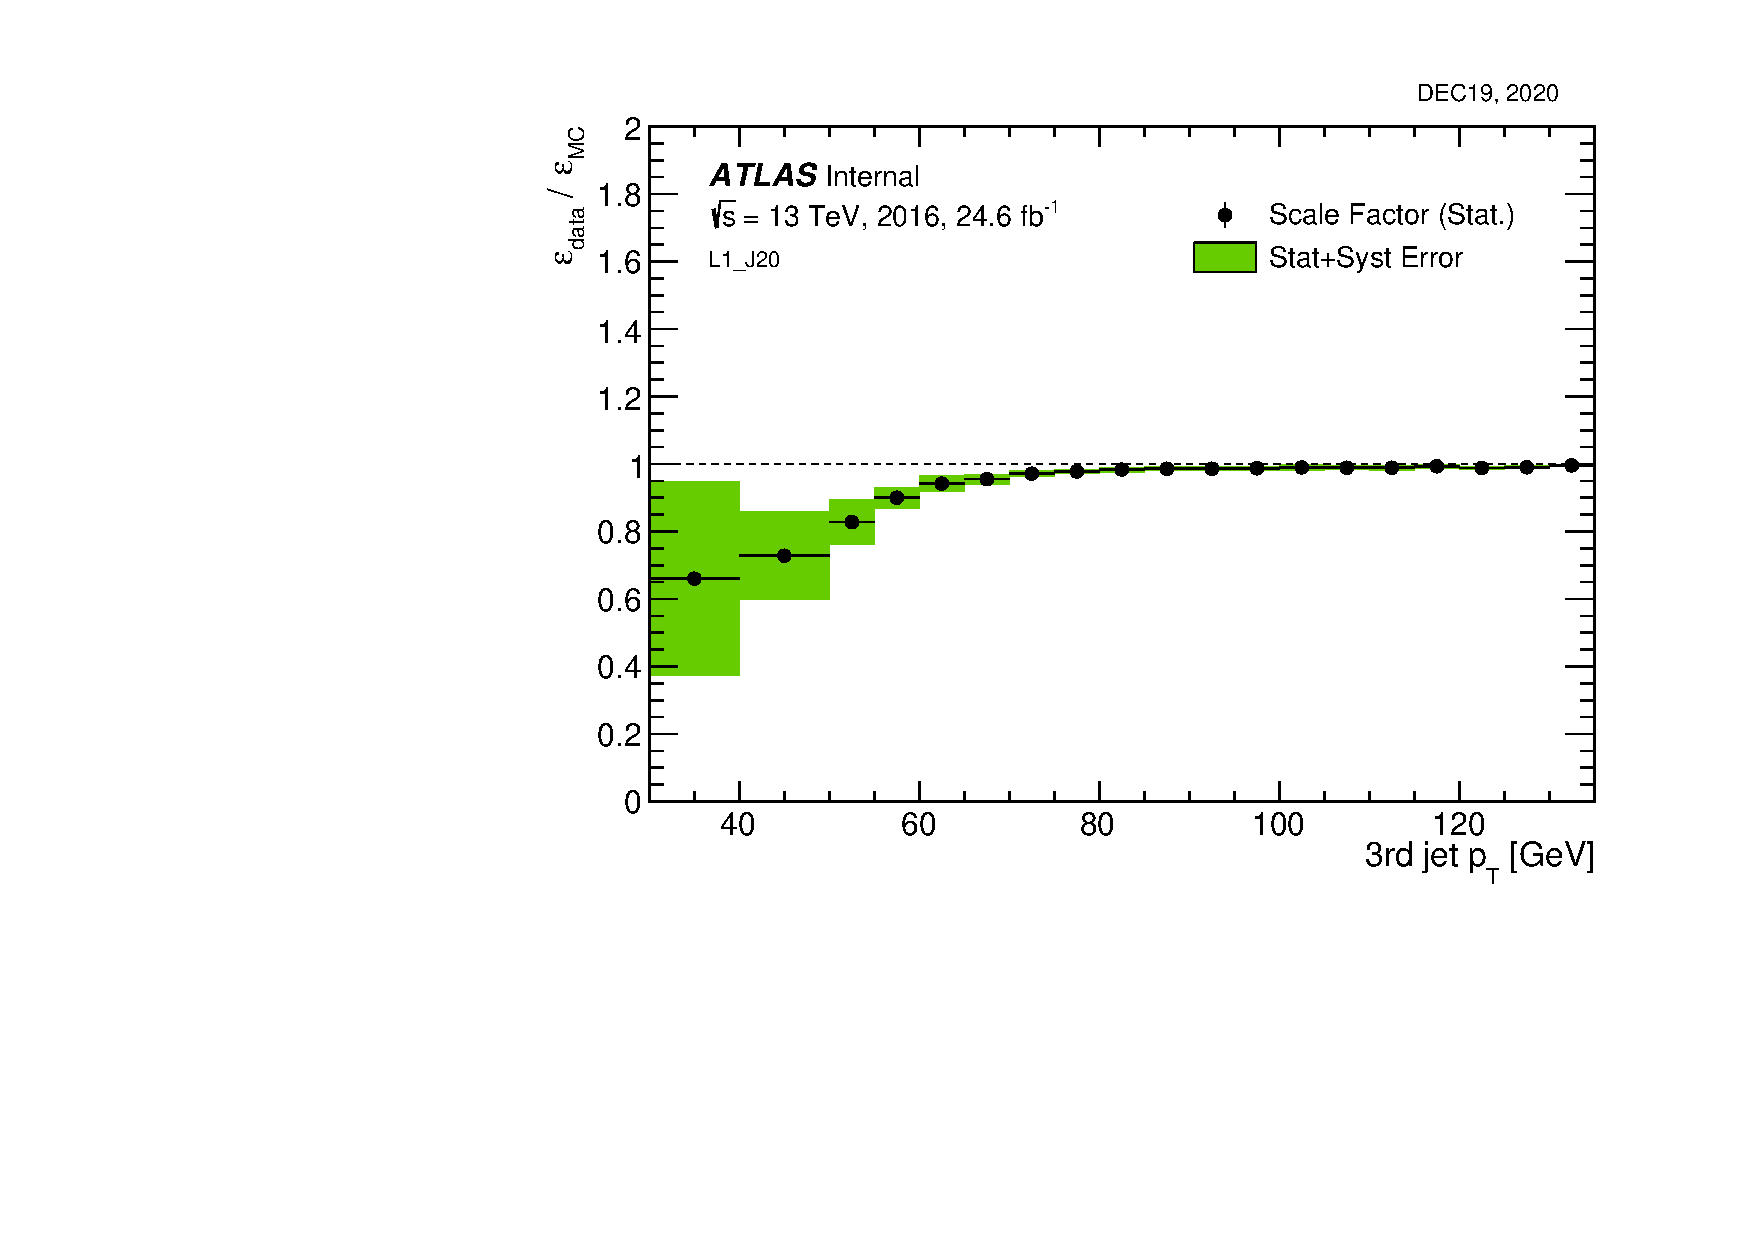
\includegraphics[width=0.25\textwidth]{\figpath{L1SF/2016/trigSF16-2b1j-L1-3rd.pdf}}
    }   
 
    \subfloat[1st jet at HLT]{\label{fig:trigSF16-2b1j-HLT-1st}%
            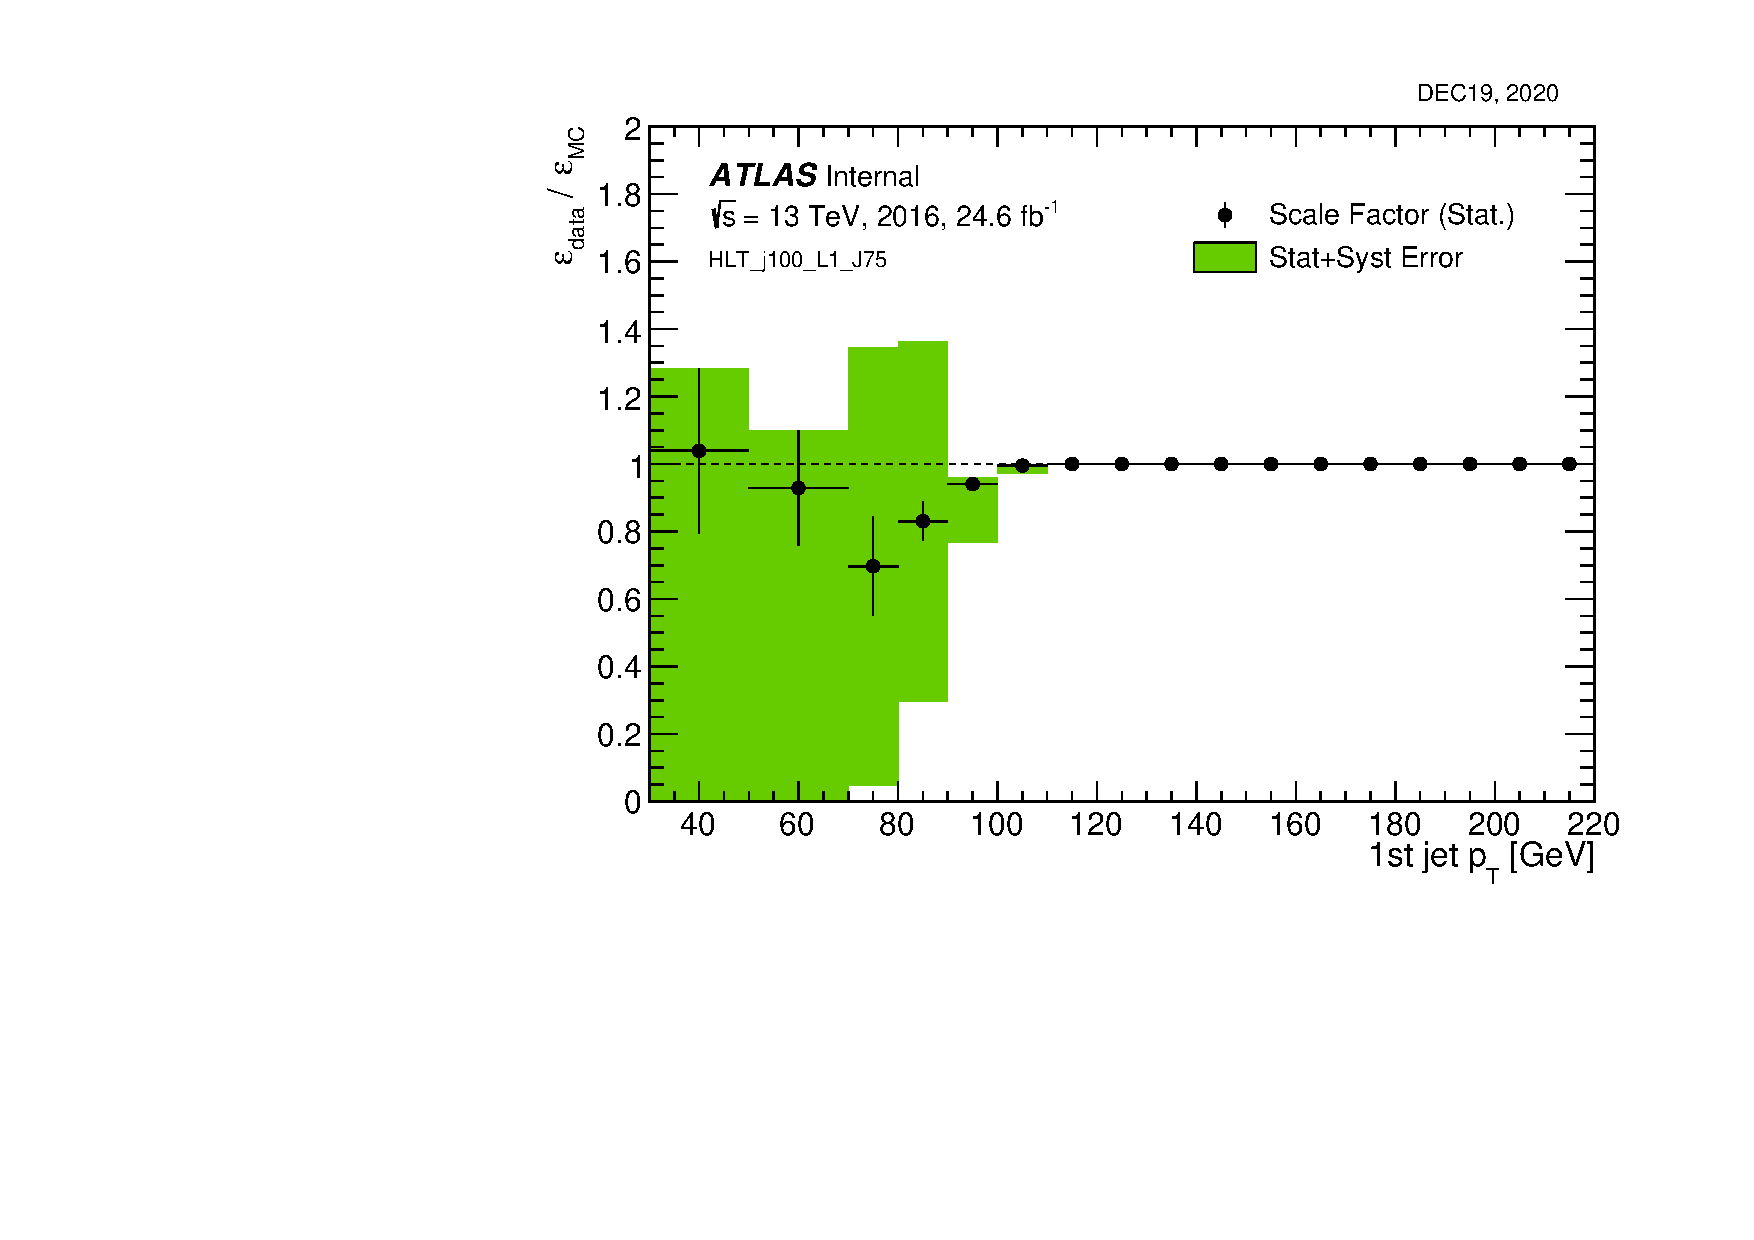
\includegraphics[width=0.25\textwidth]{\figpath{HLTSF/2016/trigSF16-2b1j-HLT-1st.pdf}}
    }   
    \subfloat[2nd jet at HLT]{\label{fig:trigSF16-2b1j-HLT-2nd}%
            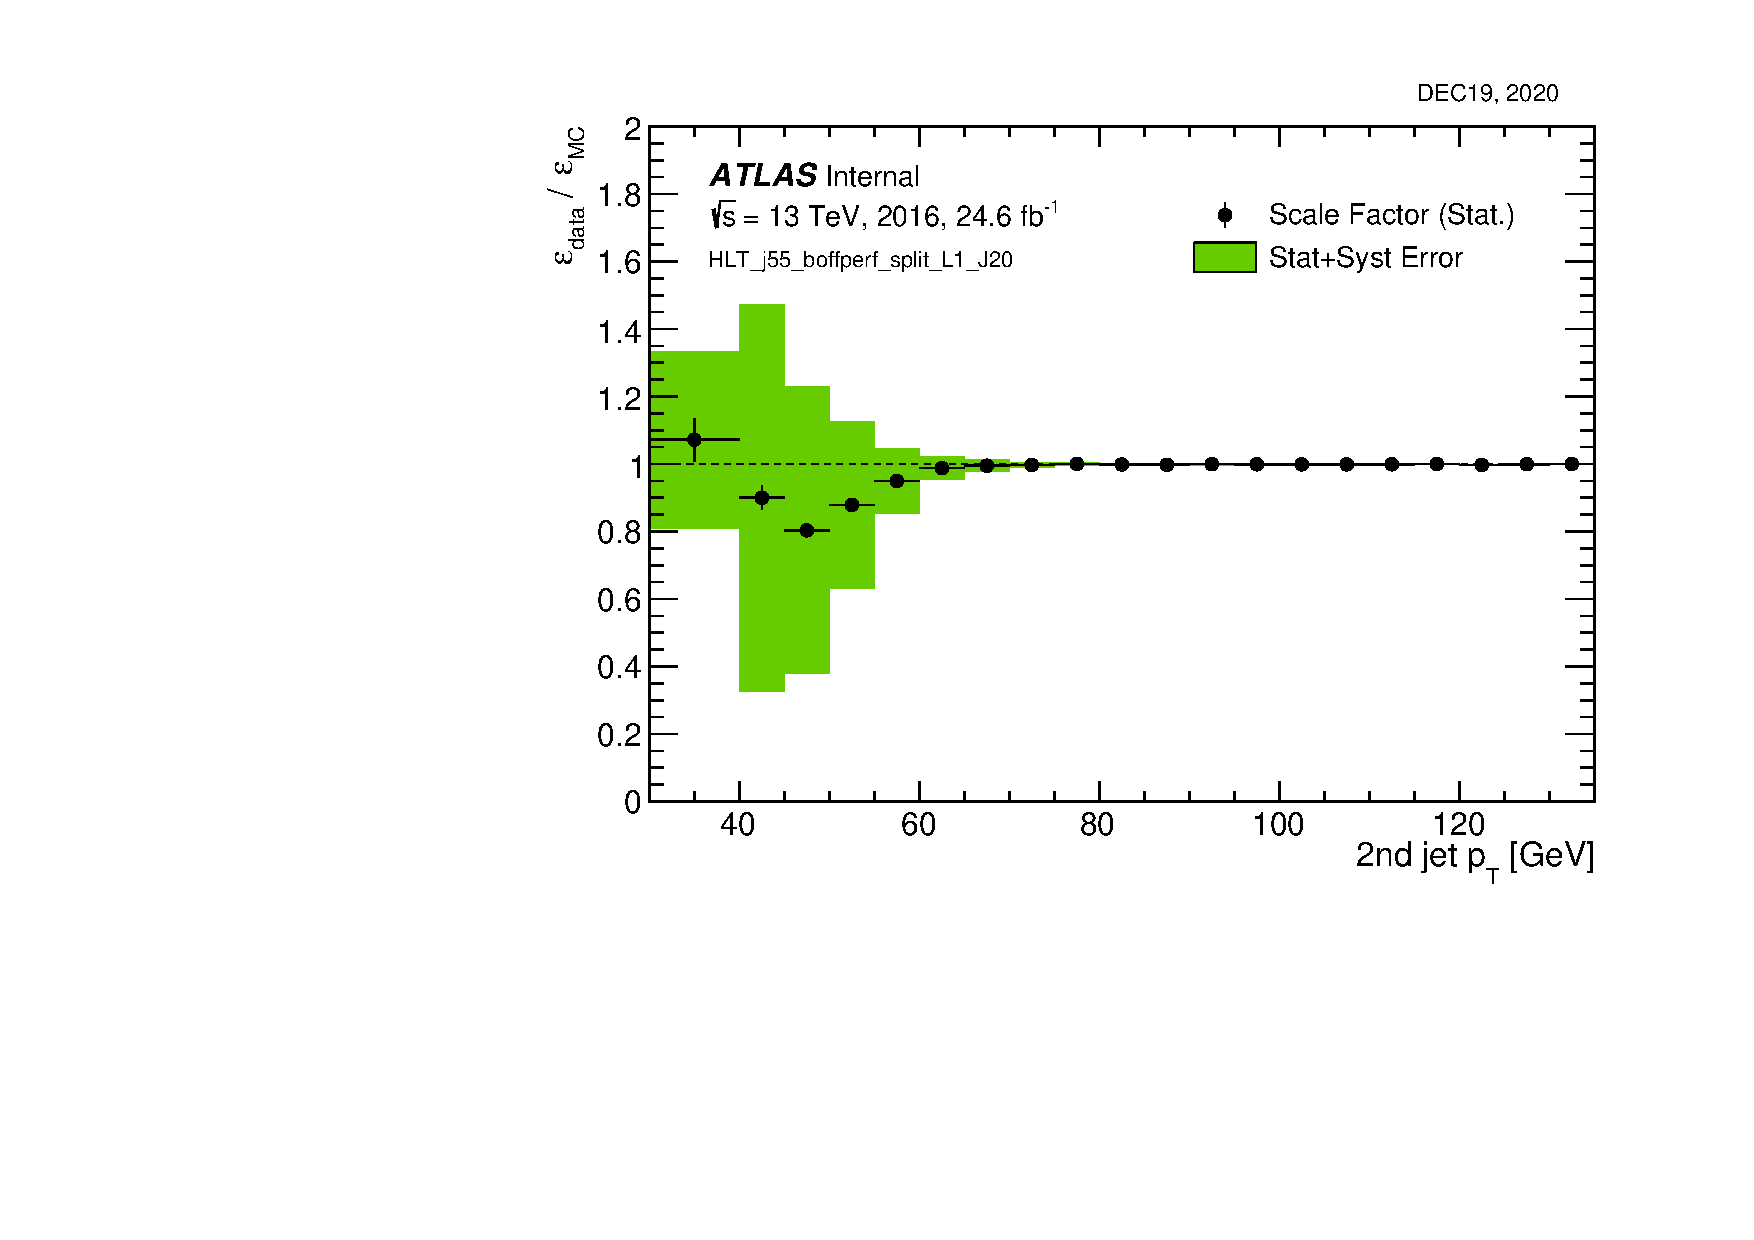
\includegraphics[width=0.25\textwidth]{\figpath{HLTSF/2016/trigSF16-2b1j-HLT-2nd.pdf}}
    }   
    \subfloat[3rd jet at HLT]{\label{fig:trigSF16-2b1j-HLT-3rd}%
            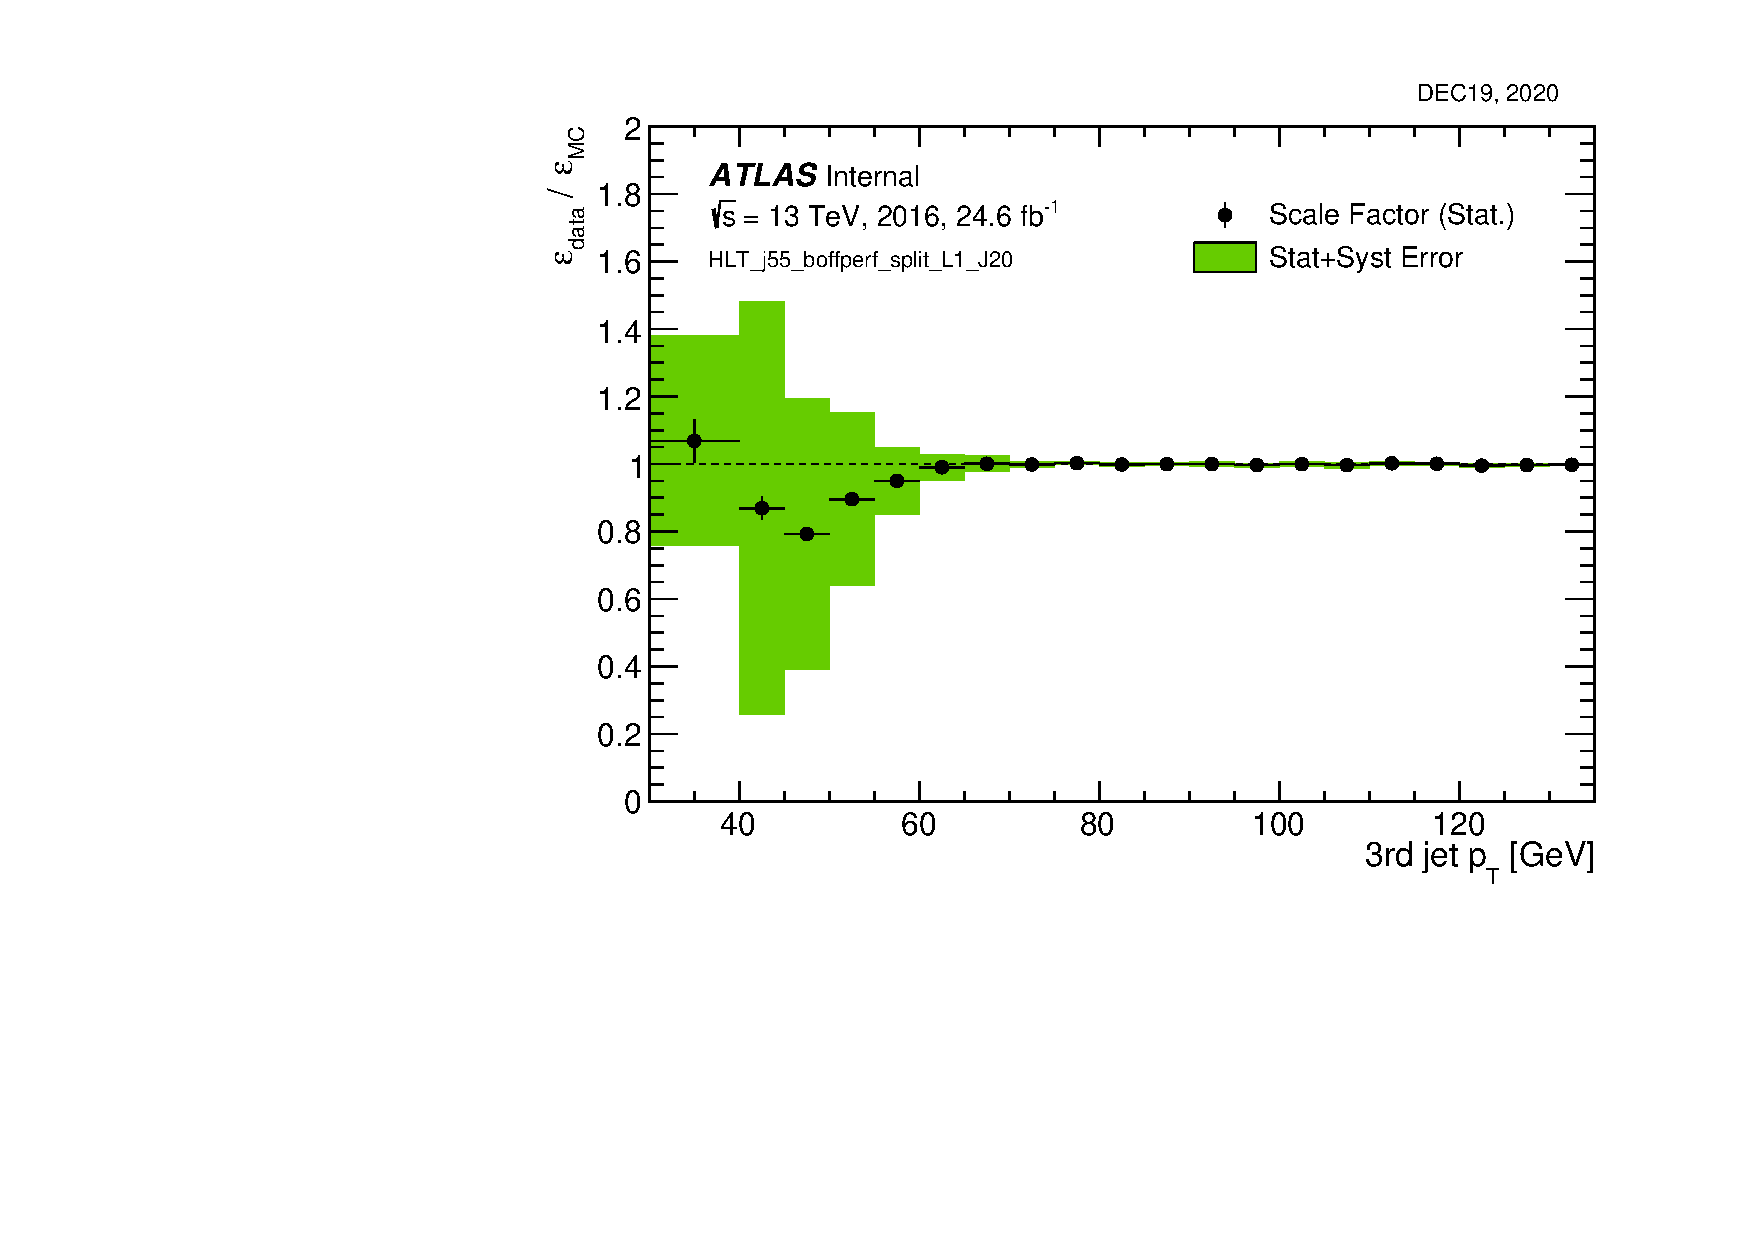
\includegraphics[width=0.25\textwidth]{\figpath{HLTSF/2016/trigSF16-2b1j-HLT-3rd.pdf}}
    }   
    \caption{Jet-level scale factors of 2016 2b1j trigger as a function of offline jet \pt.
             The Nth jet is ordered by online \et. }
    \label{fig:trigSF16-2b1j}
\end{figure}

\begin{figure}[ht]
    \centering
    \subfloat[1st jet at L1]{\label{fig:trigSF16-2b2j-L1-1st}%
            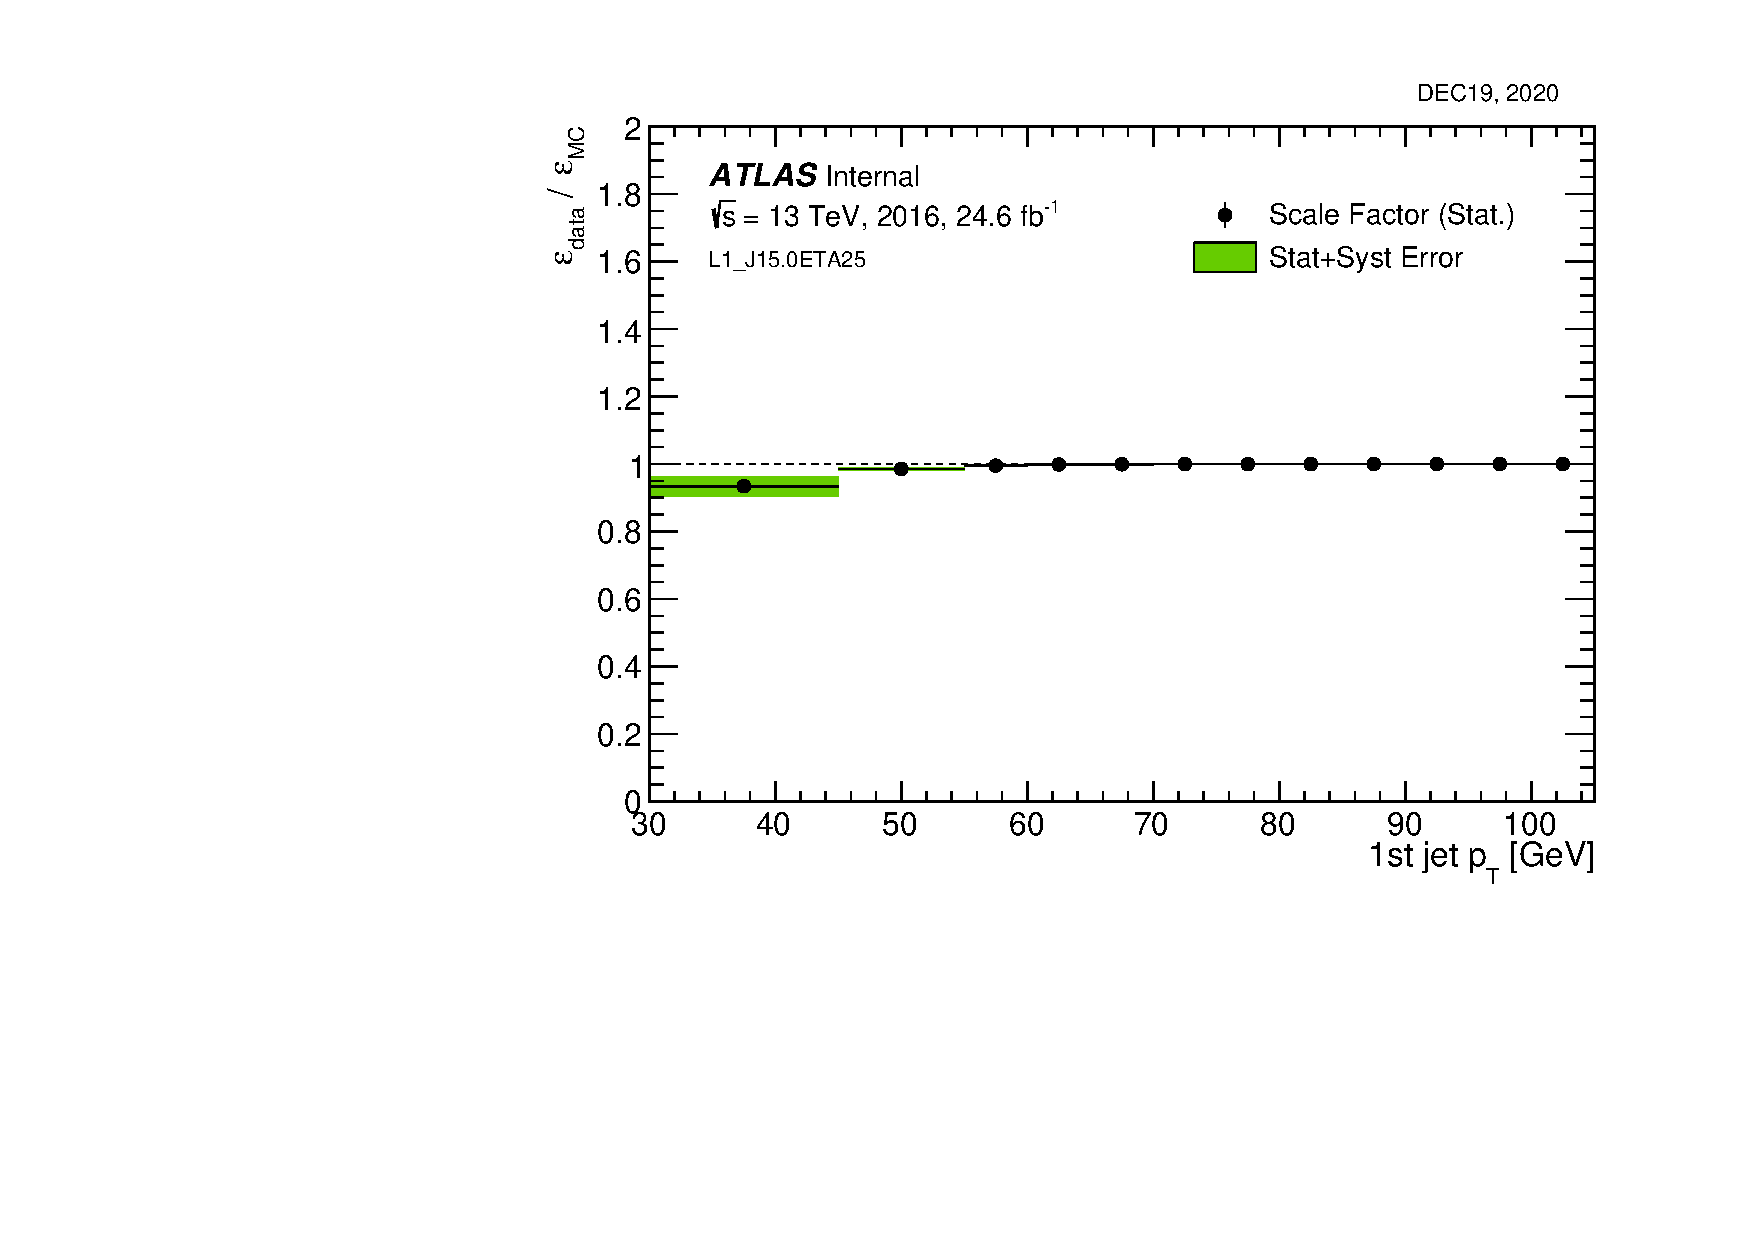
\includegraphics[width=0.25\textwidth]{\figpath{L1SF/2016/trigSF16-2b2j-L1-1st.pdf}}
    }   
    \subfloat[2nd jet at L1]{\label{fig:trigSF16-2b2j-L1-2nd}%
            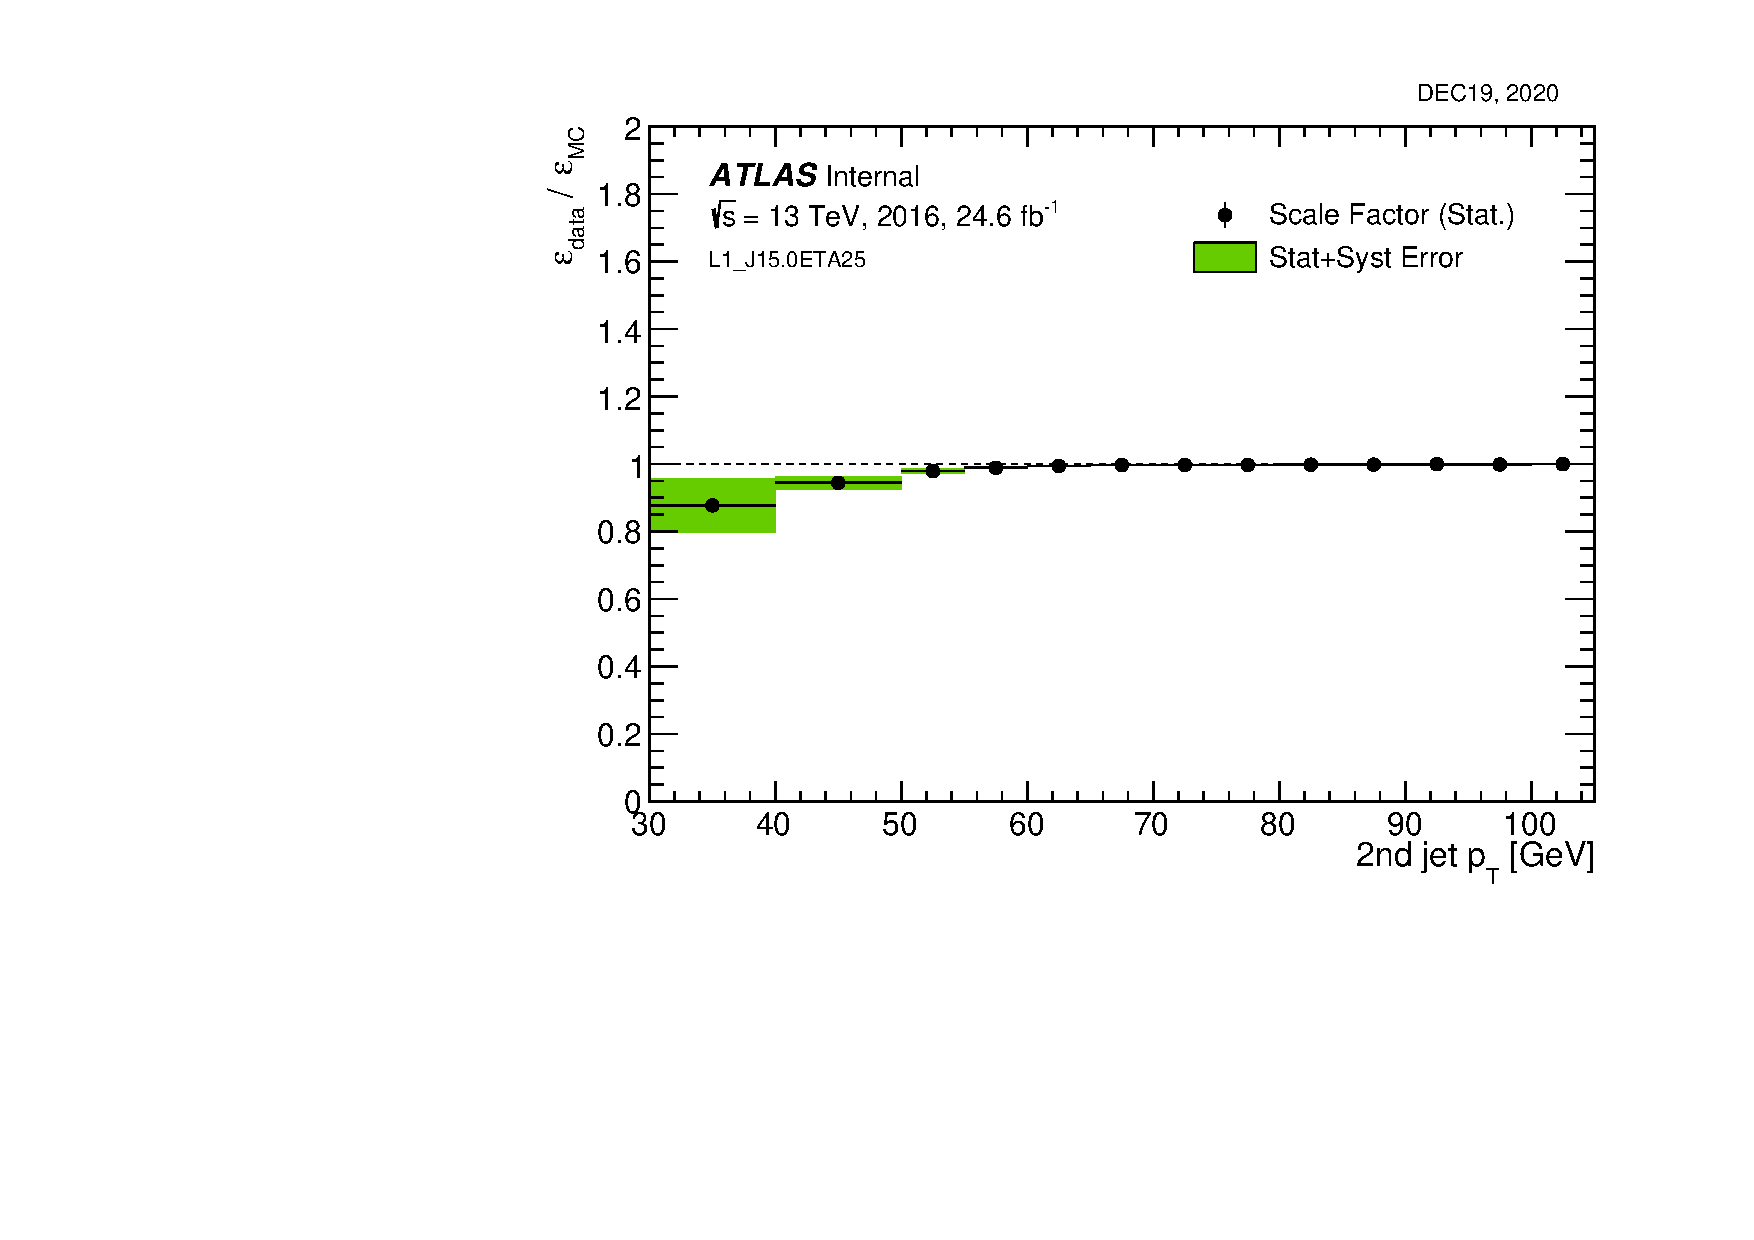
\includegraphics[width=0.25\textwidth]{\figpath{L1SF/2016/trigSF16-2b2j-L1-2nd.pdf}}
    }
    \subfloat[3rd jet at L1]{\label{fig:trigSF16-2b2j-L1-3rd}%
            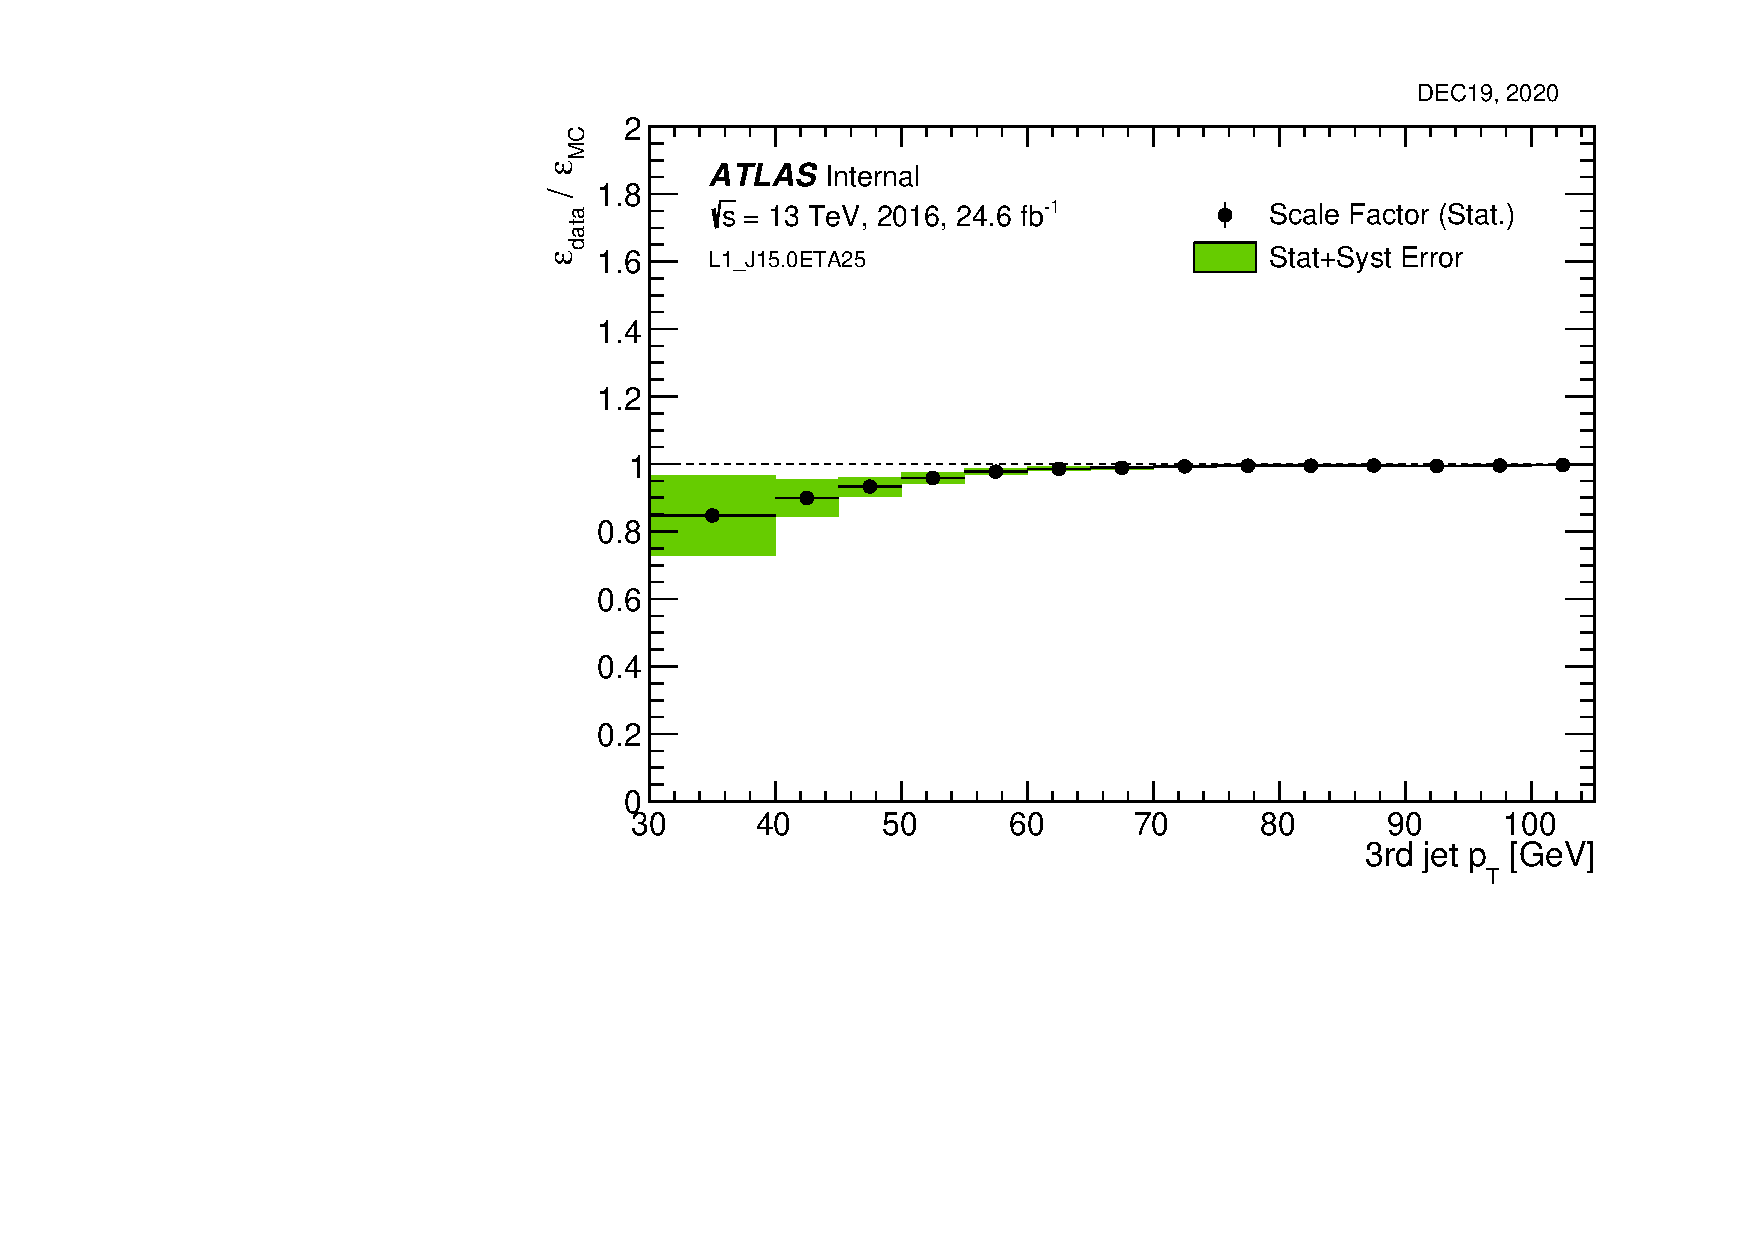
\includegraphics[width=0.25\textwidth]{\figpath{L1SF/2016/trigSF16-2b2j-L1-3rd.pdf}}
    }   
    \subfloat[4th jet at L1]{\label{fig:trigSF16-2b2j-L1-4th}%
            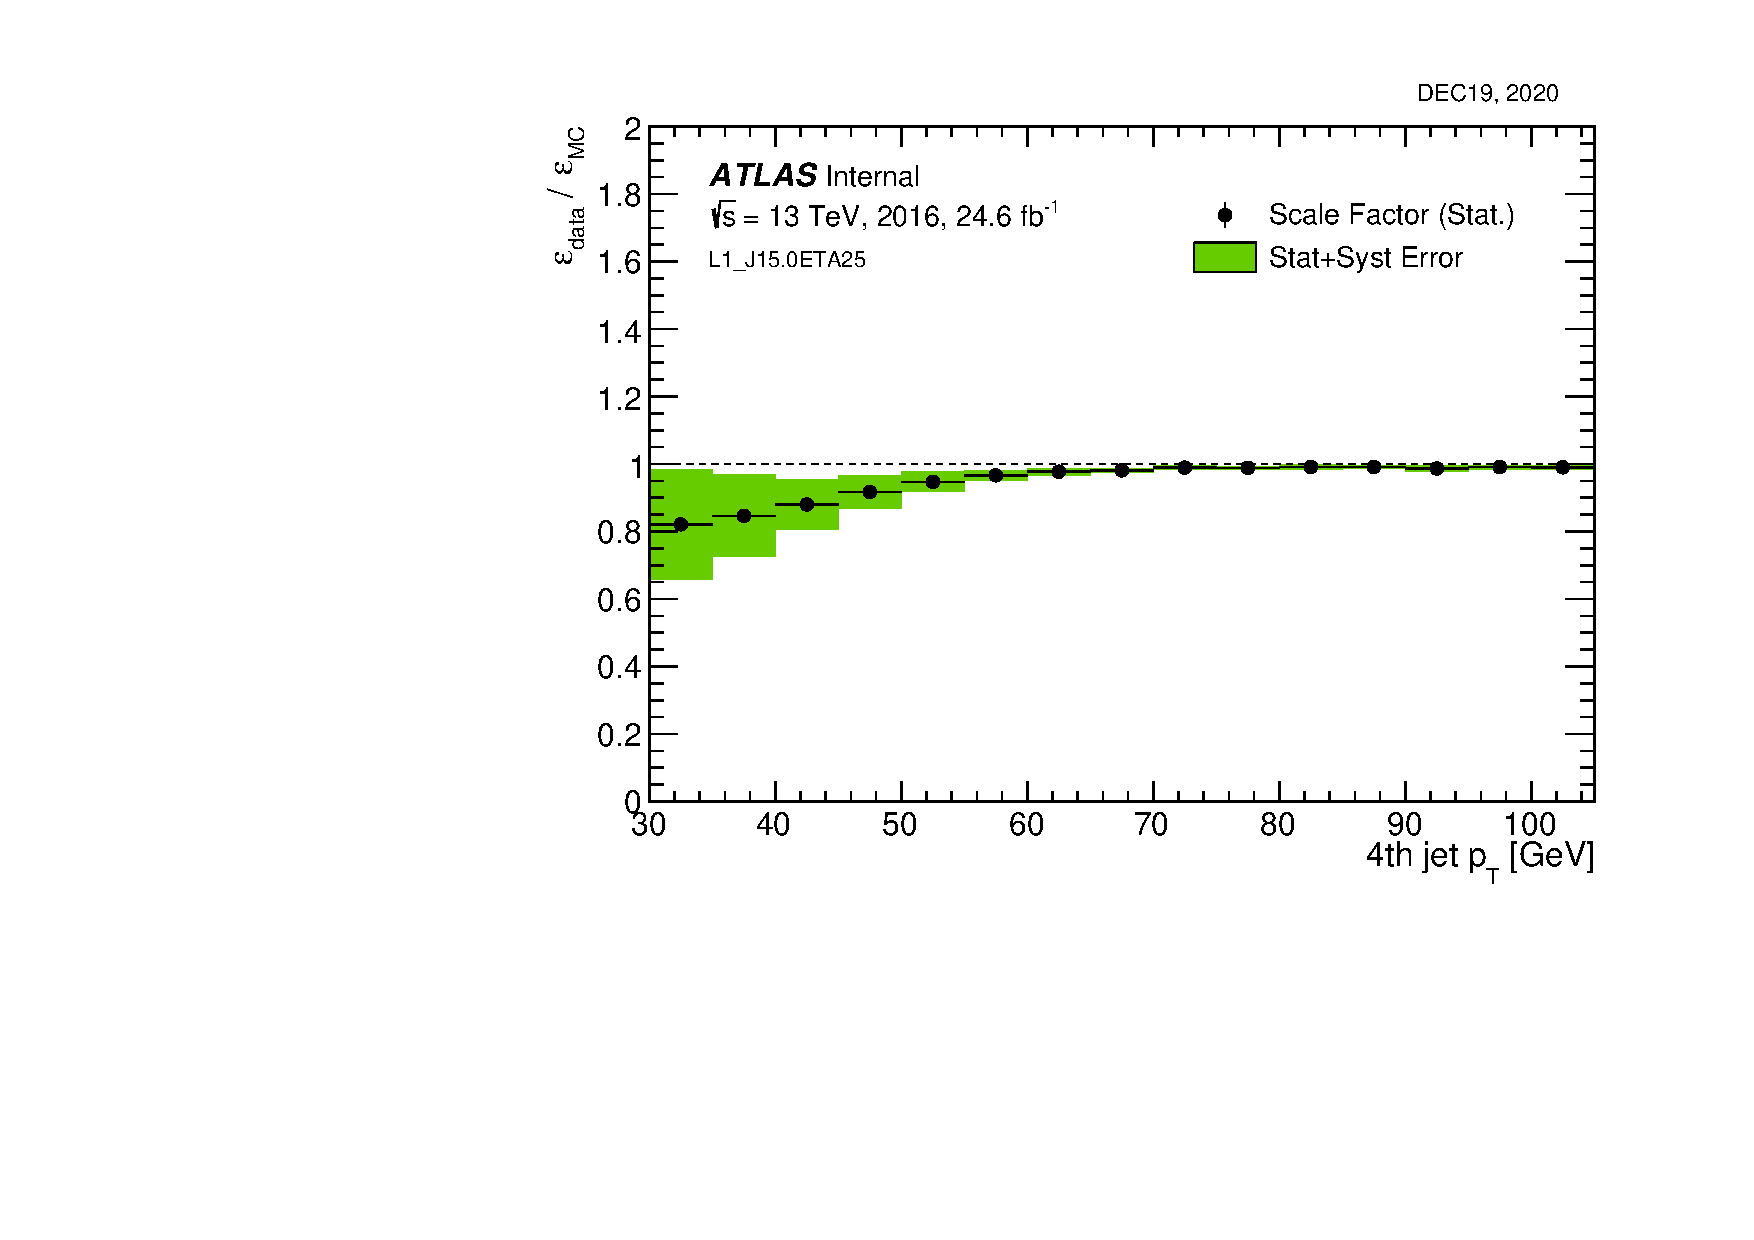
\includegraphics[width=0.25\textwidth]{\figpath{L1SF/2016/trigSF16-2b2j-L1-4th.pdf}}
    }   
   
    \subfloat[1st jet at HLT]{\label{fig:trigSF16-2b2j-HLT-1st}%
            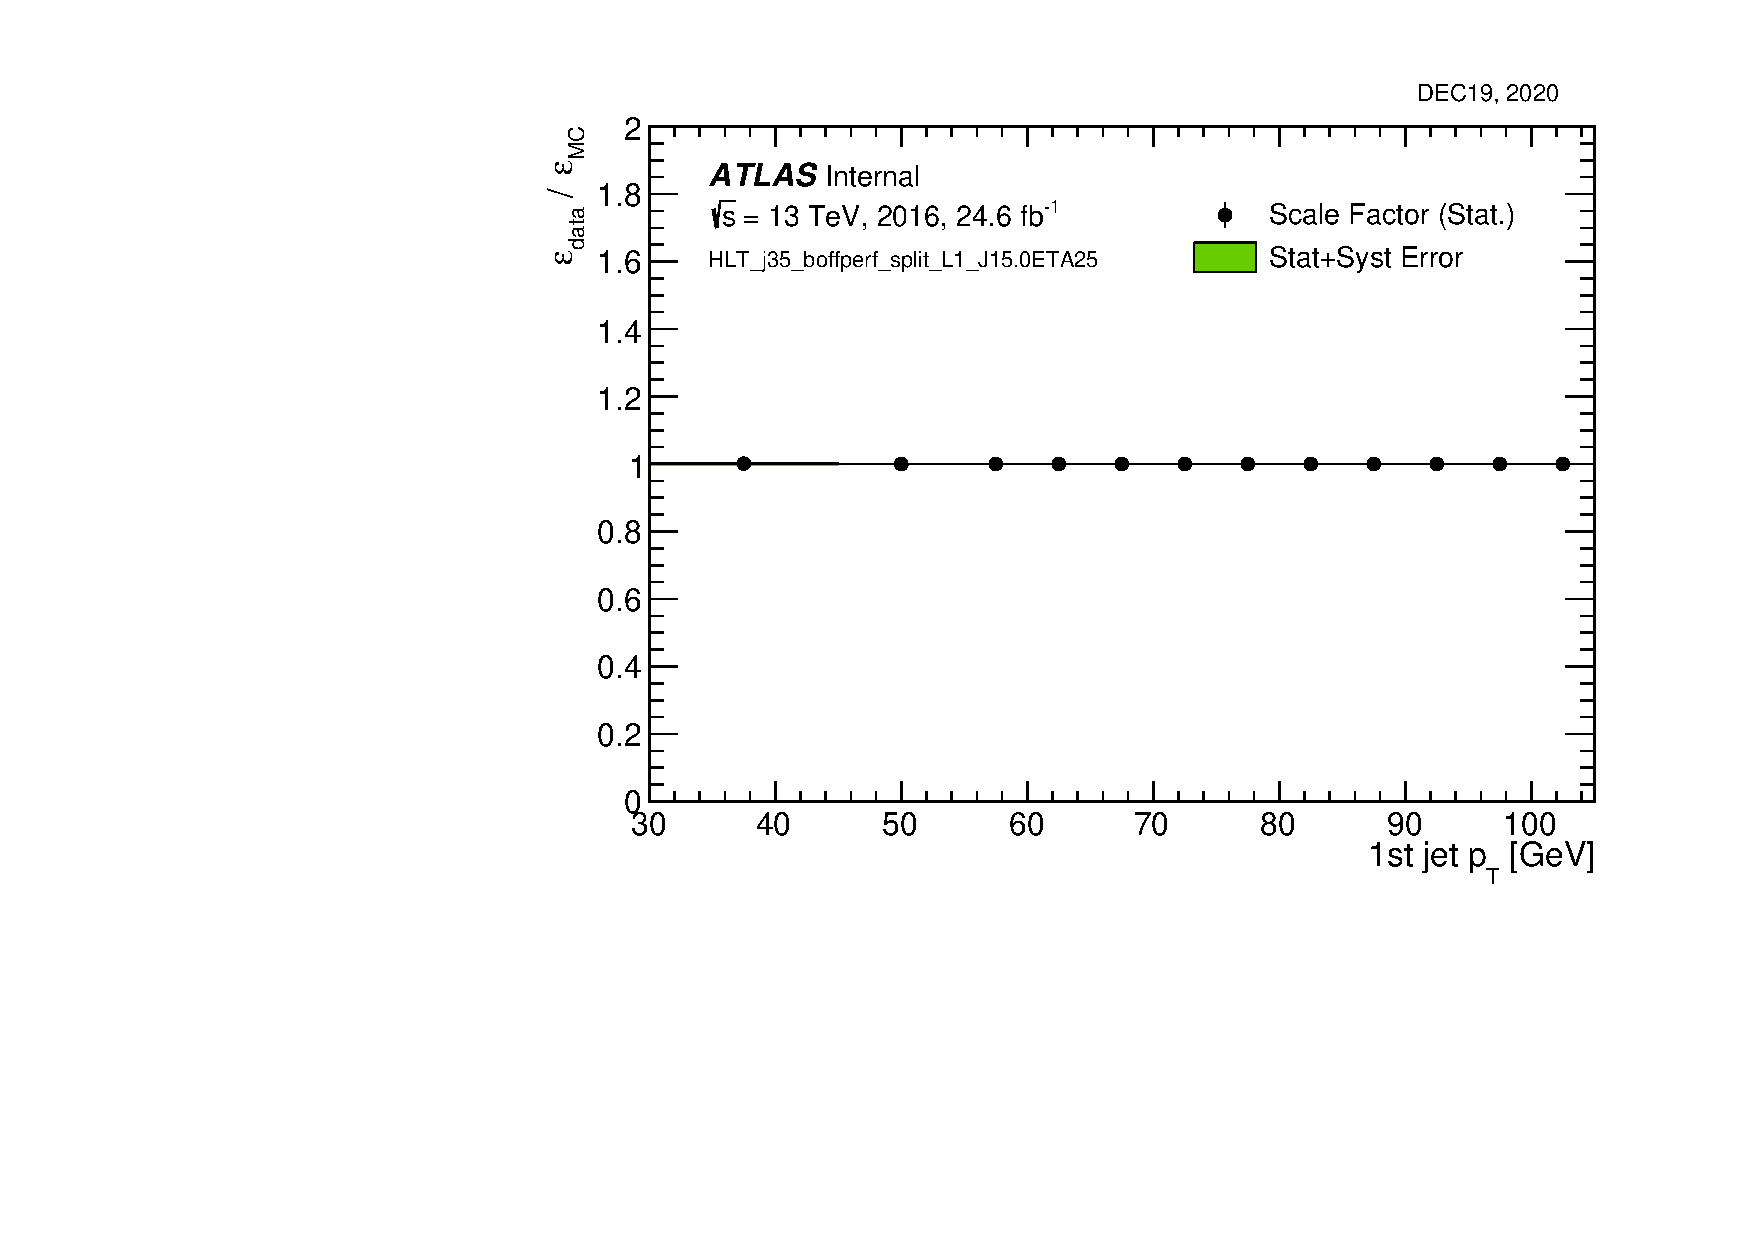
\includegraphics[width=0.25\textwidth]{\figpath{HLTSF/2016/trigSF16-2b2j-HLT-1st.pdf}}
    }   
    \subfloat[2nd jet at HLT]{\label{fig:trigSF16-2b2j-HLT-2nd}%
            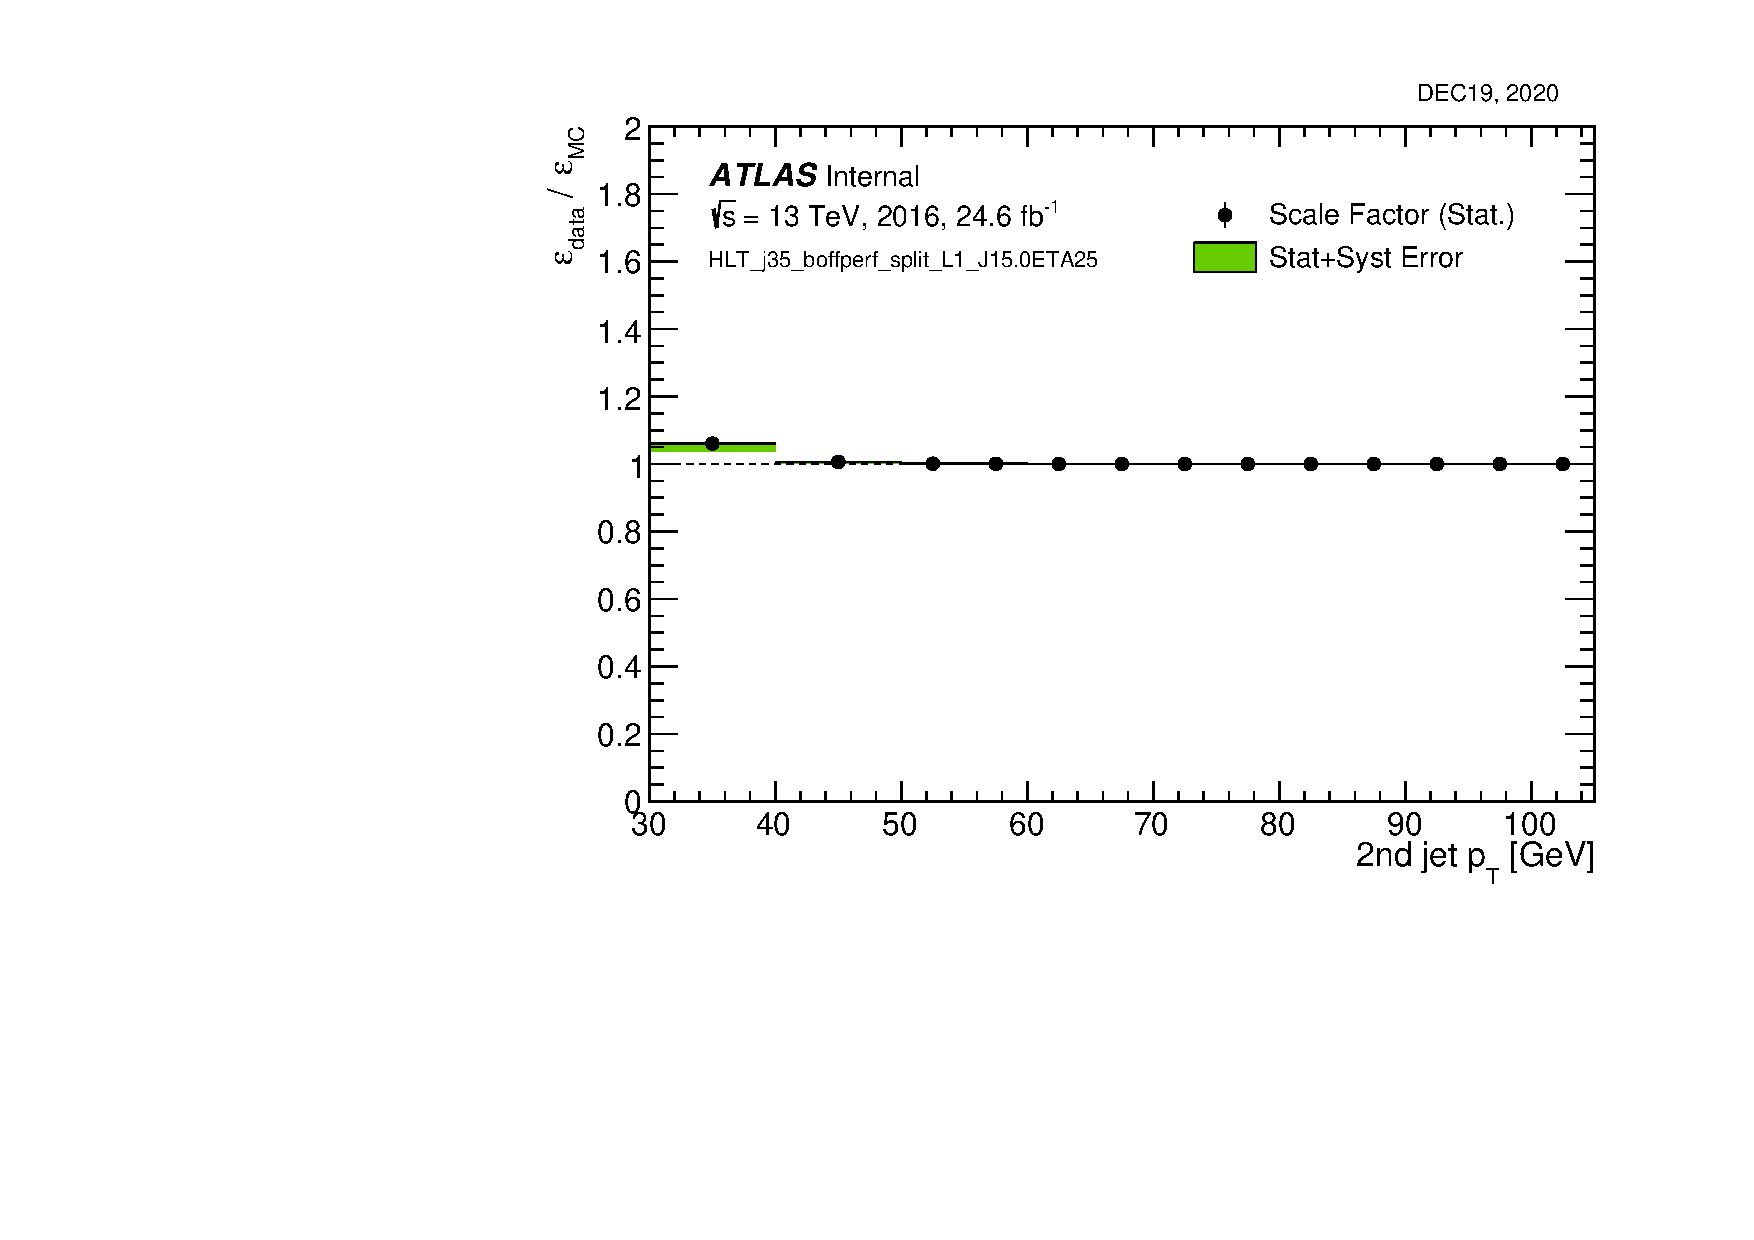
\includegraphics[width=0.25\textwidth]{\figpath{HLTSF/2016/trigSF16-2b2j-HLT-2nd.pdf}}
    }   
    \subfloat[3rd jet at HLT]{\label{fig:trigSF16-2b2j-HLT-3rd}%
            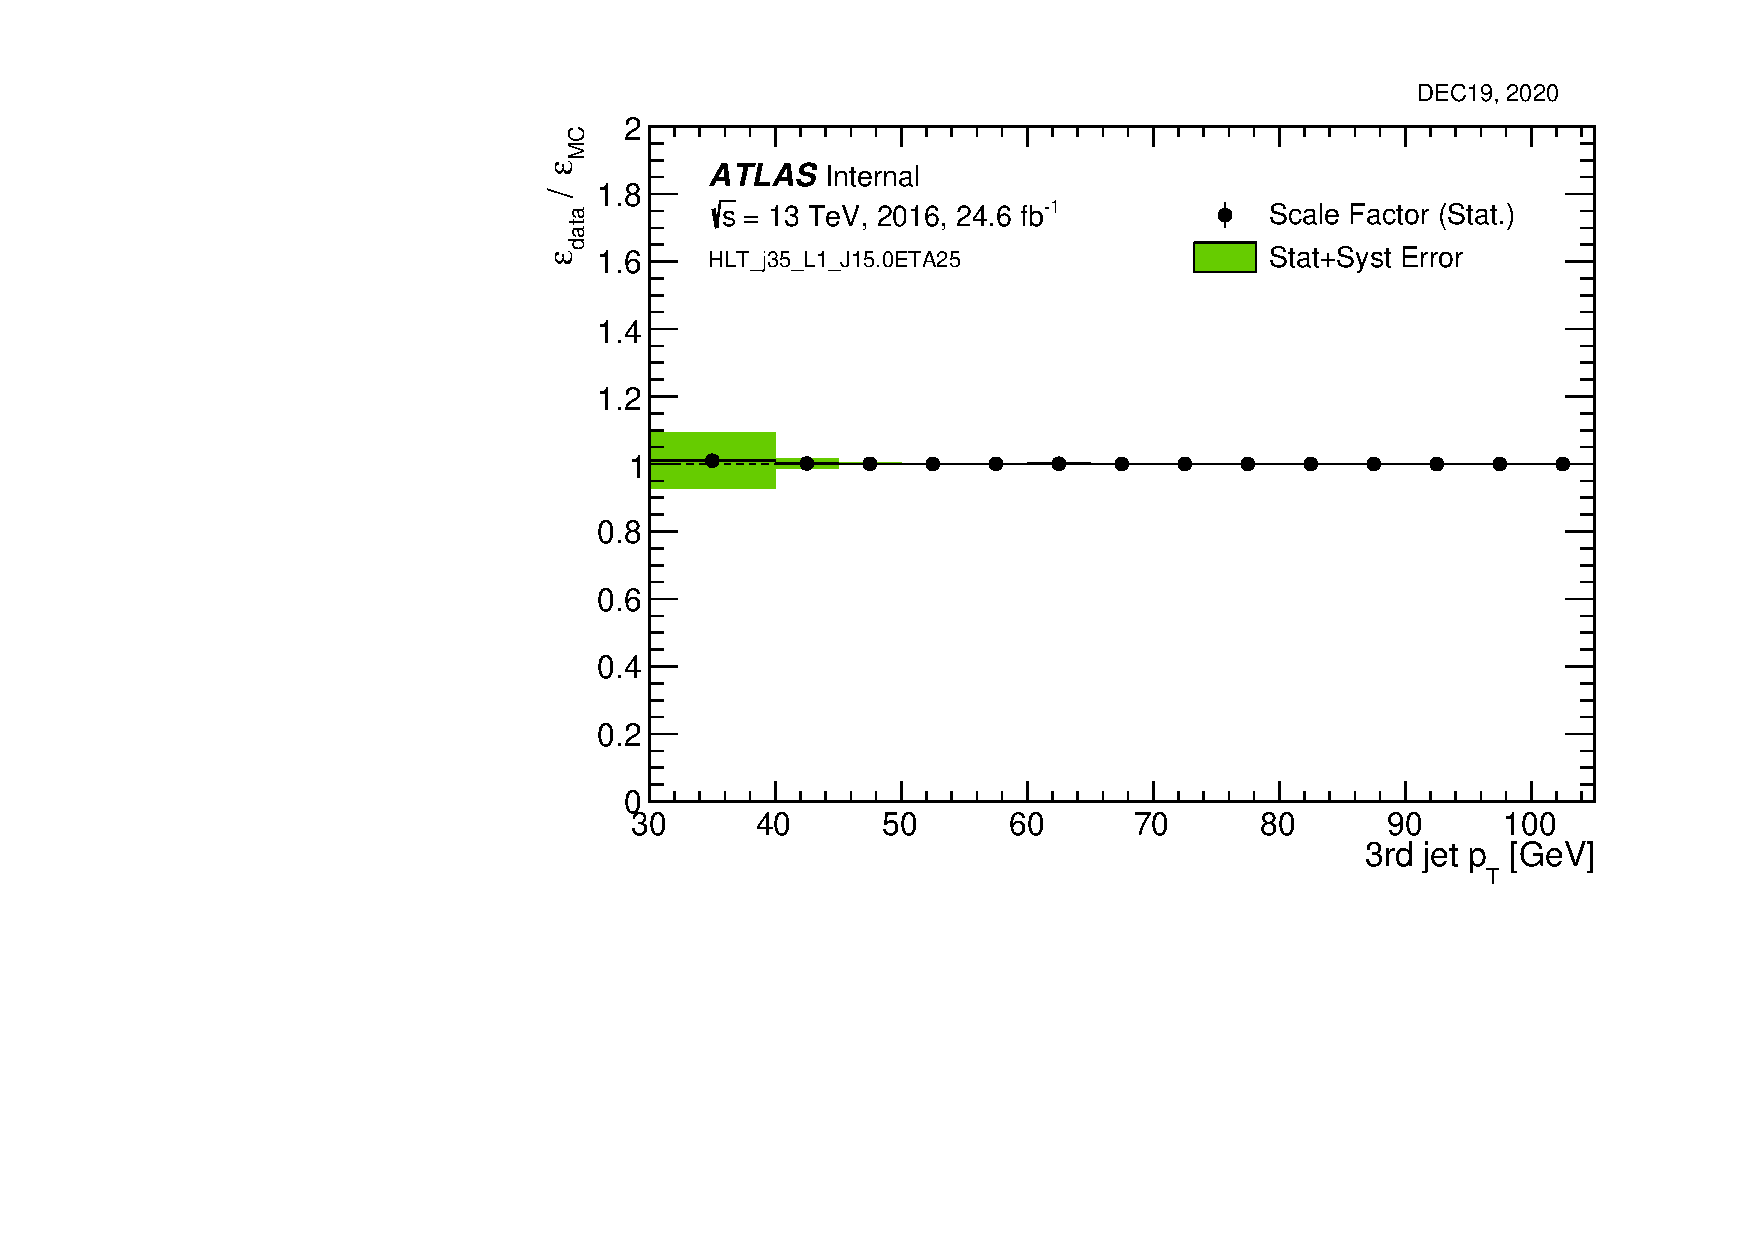
\includegraphics[width=0.25\textwidth]{\figpath{HLTSF/2016/trigSF16-2b2j-HLT-3rd.pdf}}
    }   
    \subfloat[4th jet at HLT]{\label{fig:trigSF16-2b2j-HLT-4th}%
            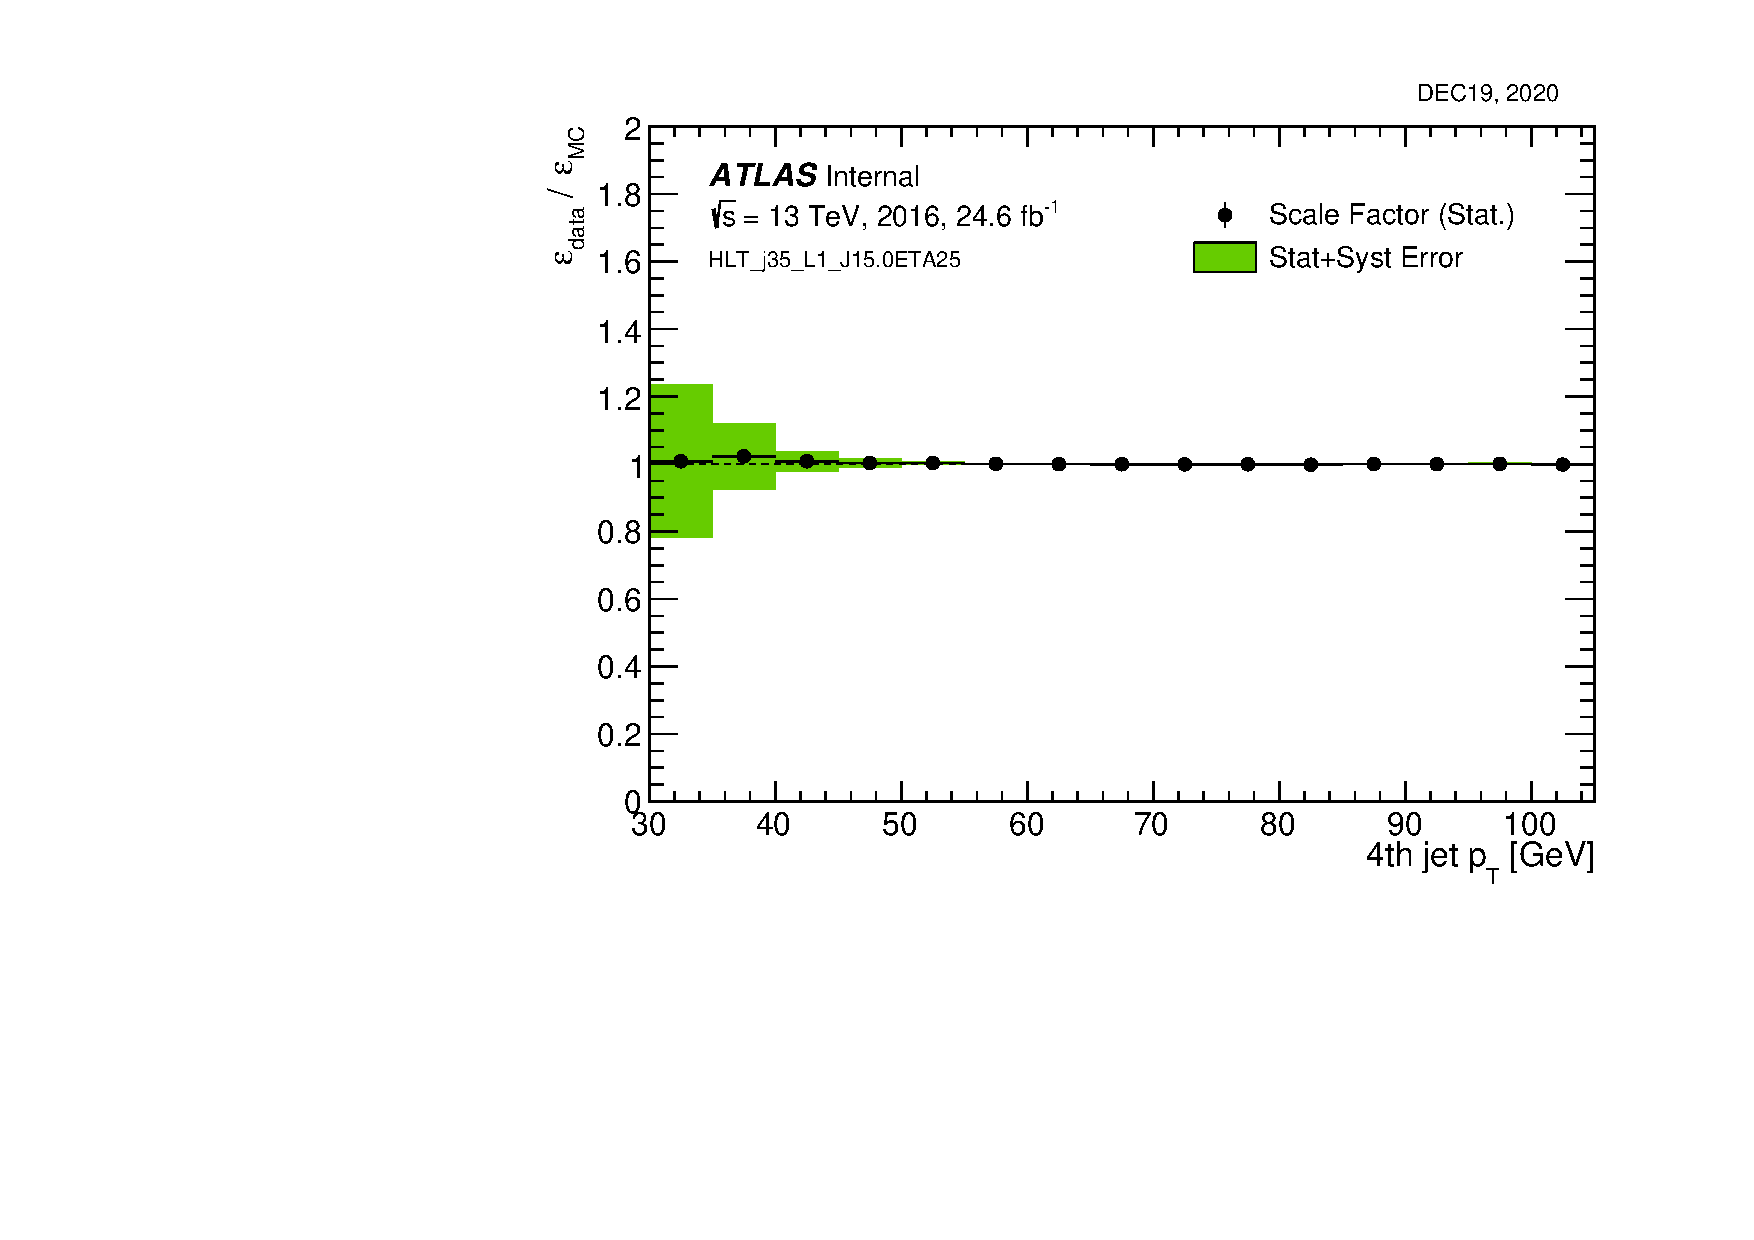
\includegraphics[width=0.25\textwidth]{\figpath{HLTSF/2016/trigSF16-2b2j-HLT-4th.pdf}}
    }   
    \caption{Jet-level scale factors of 2016 2b2j trigger as a function of offline jet \pt.
             The Nth jet is ordered by online \et. }
    \label{fig:trigSF16-2b2j}
\end{figure}

